\documentclass[
	a4paper,
	pagesize,
	pdftex,
	12pt,
	twoside, % + BCOR darunter: für doppelseitigen Druck aktivieren, sonst beide deaktivieren
	BCOR=5mm, % Dicke der Bindung berücksichtigen (Copyshop fragen, wie viel das ist)
	ngerman,
	fleqn,
	final,
	]{scrartcl}
\usepackage{ucs}
\usepackage[utf8x]{inputenc} % Eingabekodierung: UTF-8
\usepackage{fixltx2e} % Schickere Ausgabe
\usepackage[T1]{fontenc} % ordentliche Trennung
\usepackage[english]{babel}
\usepackage{lmodern} % ordentliche Schriften
\usepackage[unicode=true]{hyperref}
\usepackage{setspace,graphicx,tikz,tabularx} % für Elemente der Titelseite
\usepackage[draft=false,babel,tracking=true,kerning=true,spacing=true]{microtype} % optischer Randausgleich etc.

% figure stuff
\usepackage{caption}
\usepackage{subcaption}
\usepackage{wrapfig}

% no indent
\setlength\parindent{0pt}

% code snippet settings
\usepackage{listings}
\usepackage{color}

\definecolor{dkgreen}{rgb}{0,0.6,0}
\definecolor{gray}{rgb}{0.5,0.5,0.5}
\definecolor{mauve}{rgb}{0.58,0,0.82}

\lstset{
  frame=single,
  language=Java,
  aboveskip=3mm,
  belowskip=3mm,
  showstringspaces=false,
  columns=flexible,
  basicstyle={\small\ttfamily},
  numbers=left,
  numberstyle=\tiny\color{gray},
  keywordstyle=\color{blue},
  commentstyle=\color{dkgreen},
  stringstyle=\color{mauve},
  breaklines=true,
  breakatwhitespace=true,
  tabsize=2
}

% quotes
\usepackage[autostyle]{csquotes}

\captionsetup[figure]{slc=off}




\begin{document}

% Beispielhafte Nutzung der Vorlage für die Titelseite (bitte anpassen):
% LaTeX-Vorlage für die Titelseite und Selbständigkeitserklärung einer Abschlussarbeit
% basierend auf der vorigen Institutsvorlage des Instituts für Informatik
% sowie der Vorlage für Promotionsarbeiten.
%
% erweitert: 2014-06-12 Dennis Schneider <dschneid@informatik.hu-berlin.de>

% gepunktete Linie unter Objekt:
\newcommand{\TitelPunkte}[1]{%
  \tikz[baseline=(todotted.base)]{
    \node[inner sep=1pt,outer sep=0pt] (todotted) {#1};
    \draw[dotted] (todotted.south west) -- (todotted.south east);
  }%
}%

% gepunktete Linie mit gegebener Länge:
\newcommand{\TitelPunktLinie}[1]{\TitelPunkte{\makebox[#1][l]{}}}

\makeatletter

\newcommand*{\@titelTitel}{Titel der Arbeit}
\newcommand{\titel}[1]{\renewcommand*{\@titelTitel}{#1}} % Titel der Arbeit
\newcommand*{\@titelArbeit}{Arbeitstyp}
\newcommand{\typ}[1]{\renewcommand*{\@titelArbeit}{#1}} % Typ der Arbeit
\newcommand*{\@titelGrad}{akademischer Grad}
\newcommand{\grad}[1]{\renewcommand*{\@titelGrad}{#1}} % Akademischer Grad
\newcommand*{\@titelAutor}{Autor}
\newcommand{\autor}[1]{\renewcommand*{\@titelAutor}{#1}} % Autor der Arbeit
\newcommand*{\@titelGeburtsdatum}{\TitelPunktLinie{2cm}}
\newcommand{\gebdatum}[1]{\renewcommand*{\@titelGeburtsdatum}{#1}} % Geburtsdatum des Autors
\newcommand*{\@titelGeburtsort}{\TitelPunktLinie{5cm}}
\newcommand{\gebort}[1]{\renewcommand*{\@titelGeburtsort}{#1}} % Geburtsort des Autors
\newcommand*{\@titelGutachterA}{\TitelPunktLinie{5cm}}
\newcommand*{\@titelGutachterB}{\TitelPunktLinie{5cm}}
\newcommand{\gutachter}[2]{\renewcommand*{\@titelGutachterA}{#1}\renewcommand*{\@titelGutachterB}{#2}} % Erst- und Zweitgutachter
\newcommand*{\@titelEinreichungsdatum}{\TitelPunktLinie{3cm}} % Datum der Einreichung, wird nicht vom Studenten ausgefüllt
\newcommand*{\@titelVerteidigungsdatum}{} % Verteidigungstext, wird nicht vom Studenten ausgefüllt
\newcommand{\mitverteidigung}{\renewcommand*{\@titelVerteidigungsdatum}{verteidigt am: \,\,\TitelPunktLinie{3cm}}} % Verteidigungsplatzhalter erzeugen
\newcommand*{\@wastwoside}{}

% Titelseite erzeugen:
\newcommand{\makeTitel}{%
	% Speichere, ob doppelseitiges Layout gewählt wurde:
\if@twoside%
	\renewcommand*{\@wastwoside}{twoside}
\else
	\renewcommand*{\@wastwoside}{twoside=false}
\fi
	\KOMAoptions{twoside = false}% Erzwinge einseitiges Layout (erzeugt eine Warnung)

	\begin{titlepage}
		% Ändern der Einrückungen
		\newlength{\parindentbak} \setlength{\parindentbak}{\parindent}
		\newlength{\parskipbak} \setlength{\parskipbak}{\parskip}
		\setlength{\parindent}{0pt}
		\setlength{\parskip}{\baselineskip}

		\thispagestyle{empty}

		\begin{minipage}[c][3cm][c]{12cm}
			\textsc{%
				% optischer Randausgleich per Hand:
				\hspace{-0.4mm}\textls*[68]{\Large Humboldt-Universität zu Berlin}\\
				\normalsize \textls*[45]{
					Mathematisch-Naturwissenschaftliche Fakultät\\
					Institut für Informatik
				}
			}
		\end{minipage}
		\hfill
		\begin{minipage}[c][3cm][c]{3cm}
			
\includegraphics[width=3cm]{husiegel.pdf}
		\end{minipage}

		% Also wenn schon serifenlose Schriften (Titel), dann ganz oder gar nicht
		\sffamily

		\vfill

		\begin{center}
		\begin{doublespace}
			\vspace{\baselineskip}
			{\LARGE \textbf{\@titelTitel}}\\
			%\vspace{1\baselineskip}
			{\Large
				\@titelArbeit\\
				zur Erlangung des akademischen Grades\\
				\@titelGrad
				\vspace{\baselineskip}
			}
		\end{doublespace}
		\end{center}

		\vfill
\newcolumntype{L}{>{\raggedright\arraybackslash}X}
		{\large \raggedleft
			\begin{tabularx}{\textwidth}{l@{\,\,\raggedright~}L} % verbreiterter Abstand zwischen Feldern wurde gewünscht
				eingereicht von: & \@titelAutor\\
				geboren am: & {\@titelGeburtsdatum}\\
				geboren in: & \@titelGeburtsort
				\vspace{0.5\baselineskip}\\
				Gutachter/innen: & \@titelGutachterA \\
					& \@titelGutachterB
				\vspace{0.5\baselineskip}\\
				eingereicht am: & \@titelEinreichungsdatum \hfill \@titelVerteidigungsdatum
			\end{tabularx}}
			\vspace{-1\baselineskip}\\\phantom{x} % Übler Hack, um eine Warnung wg. einer zu leeren hbox zu verhindern
		% Wiederherstellen der Einrückung
		\setlength{\parindent}{\parindentbak}
		\setlength{\parskip}{\parskipbak}
	\end{titlepage}

	% Aufräumen:
	\let\@titelTitel\undefined
	\let\titel\undefined
	\let\@titelArbeit\undefined
	\let\typ\undefined
	\let\@titelGrad\undefined
	\let\grad\undefined
	\let\@titelAutor\undefined
	\let\autor\undefined
	\let\@titelGeburtsdatum\undefined
	\let\gebdatum\undefined
	\let\@titelGeburtsort\undefined
	\let\gebort\undefined
	\let\@titelGutachterA\undefined
	\let\@titelGutachterB\undefined
	\let\gutachter\undefined
	\let\@titelEinreichungsdatum\undefined
	\let\einreichungsdatum\undefined
	\let\@titelVerteidigungsdatum\undefined
	\let\verteidigungsdatum\undefined

	\KOMAoptions{\@wastwoside}% Stelle alten Modus (ein-/doppelseitig) wieder her
	\let\@wastwoside\undefined
	\cleardoublepage % ganzes Blatt für die Titelseite
}

% Als Allerallerletztes kommt Selbständigkeitserklärung:
% Aufruf mit dem Datum in deutscher und englischer Form
\newcommand{\selbstaendigkeitserklaerung}[1]{%
	\cleardoublepage% Wieder auf eine eigene Doppelseite
	{\parindent0cm
		\subsection*{Selbständigkeitserklärung}
		Ich erkläre hiermit, dass ich die vorliegende Arbeit selbständig verfasst
		und noch nicht für andere Prüfungen eingereicht habe.
		Sämtliche Quellen einschließlich Internetquellen, die unverändert oder
		abgewandelt wiedergegeben werden, insbesondere Quellen für Texte, Grafiken,
		Tabellen und Bilder, sind als solche kenntlich gemacht. Mir ist bekannt,
		dass bei Verstößen gegen diese Grundsätze ein Verfahren wegen
		Täuschungsversuchs bzw. Täuschung eingeleitet wird.
		\vspace{3\baselineskip}

		{\raggedright Berlin, den #1 \hfill \TitelPunktLinie{8cm}\\}
% Bitte verwenden Sie diese Erklaerung auch fuer englischsprachige Arbeiten. Eine Uebersetzung ist nicht zweckmaessig.
	}
}%

\makeatother



\titel{Drift: an imperative programming environment for the cloud} % Titel der Arbeit
\typ{Masterarbeit} % Typ der Arbeit:  Diplomarbeit, Masterarbeit, Bachelorarbeit
\grad{Master of Science (M. Sc.)} % erreichter Akademischer Grad
% z.B.: Master of Science (M. Sc.), Master of Education (M. Ed.), Bachelor of Science (B. Sc.), Bachelor of Arts (B. A.), Diplominformatikerin
\autor{Frank Lange} % Autor der Arbeit, mit Vor- und Nachname
\gebdatum{08.08.1989} % Geburtsdatum des Autors
\gebort{Berlin} % Geburtsort des Autors
\gutachter{Prof. Dr. Jens-Peter Redlich}{Prof. Dr. Joachim Fischer} % Erst- und Zweitgutachter der Arbeit
\mitverteidigung % entfernen, falls keine Verteidigung erfolgt
\makeTitel

% Hier folgt die eigentliche Arbeit (bei doppelseitigem Druck auf einem neuen Blatt):
\tableofcontents
\thispagestyle{empty}


\newpage
\thispagestyle{empty}
\ \\

\newpage
\thispagestyle{empty}

\vspace*{\fill}
\begin{quote}
\centering
\textit{``If I had more time, I would have written a shorter letter.''}
\\
\ \\
-- Blaise Pascal
\end{quote}
\vspace*{\fill}

\newpage
\thispagestyle{empty}
\ \\

\newpage

\section{Introduction}
Alongside the advent of multi-core CPU architectures
and increased local storage capacities, large scale distributed
systems based on commodity hardware, accommondated for in special
facilities like data centers, have proven to be a viable tool for
dealing with the ever increasing demand of compute power and
storage.

One of the largest drivers of this demand is of course
the modern web, including not only all the data accumulation
that is taking place on social networks and social media but also
providing different kinds of large scale services and platforms
like maps and navigations but also e-commerce platforms which
today include music and video streaming platforms like
\textit{Spotify}, \textit{Netflix} or \textit{Amazon Prime Music} or
\textit{Amazon Prime Video} or even transportation-on-demand
platforms like \textit{Uber}.

Additionally, the advent of artificial intelligence and
machine learning created its own demand for ever increasing
large scale neural networks and training data sets. A progression
that is deeply coupled with the products of the modern web,
providing not only recommondation or prediction engines for
the users but also scheduling and load balancing decisions
inside the systems, perfectly adapted to the given workload,
which allow to fully utilize a given system to capacity without
human intervention.
\newline

Therefore, in order to provide systems that allow to scale to millions
or even billions of users, either in terms of storage, computing,
training neural networks or simply content delivery and response times,
large scale distributed systems have been constructed which pose new
system design challenges not only regarding fault tolerance, network failure
and fail over strategies but also in terms of simply how to
describe, express and comprehend these vast and infinitely
complex systems.








\subsection{Goal of this work}
To face these challenges and to analyze and explore the
concepts needed by software engineers to describe, construct and program
these system, the following work presents the
\textit{Drift Programming Environment}, a collection of different
components that allow the programming and orchestration of a
distributed system of autonomous services by describing
their data dependencies.

The goal of this work is to not only present each individual
component of the final result, which includes an abstract,
imperative and stateful coordination language, an immutable
file system based on distributed message queues and an interactive
user interface based on the syntax of Petri Nets,
but also to introduce the reader to the set of projects and the
people that created these projects, and their ideas and philosophies,
that served as inspirations and guidance for the ideas and design decisions
included in the \textit{Drift} project.





\subsection{Structure of this work}
This is done by giving a short summary of the history and
evolution of programming languages and their adaption to
fundamental changes of the underlying hardware, especially the
advent of distributed systems in chapter \ref{distributedprogramming}.

Chapter \ref{relatedwork} then succesively introduces the related
projects and tries to extract and hightlight their relevant aspects
to the \textit{Drift} project.

Chapter \ref{drift} then introduces the components of the
\textit{Drift Programming Environment} by first introducing the
Drift language in chapter \ref{driftlang} including its implementation
in form the of the Drift shell. This is followed by the introduction
of the Drift system implementation in chapter
\ref{driftimplementation} including an extensive explanation of
the error model and distributed error handling procedure.
Finally, chapter \ref{driftui} presents the Drift UI prototype
which features the Drift shell as introduced in chapter \ref{driftshell}
as well as an interactive graphical representation of the
current state of the entire system using the Petri Net syntax
and an event time line that allows to effortlessly review previews
system states.

Chapter \ref{summary} then summarizes the presented work, including
all the presented components and their contribution to the overall
system and chapter \ref{futurework} thoroughly discusses possible
improvements regarding the implementation of each individual component
as it was introduced in chapter \ref{drift} as well as possible
progressions of future projects.

\section{Distributed Programming}
In 1937 a paper titled \textit{``On computable numbers, with an
application to the Entscheidungsproblem''}, written by Alan Turing, was
published \cite{turingcomputable}. In it Turing defines what is now
known as a \textit{Turing machine}, a theoretical machine model for
executing arbitrary computation. He demonstrates how to formulate
instructions for this machine in order to configure its execution
behavior and goes so far as to show how this
machine could even receive another machine configuration as its input
and then execute what the other machine would have done, thereby
effectively emulating the given machine.
\newline

But he wasn't the only one thinking about computation. As summarized
by Denning in \cite{whatiscomputation}, Kurt Gödel, Alonzo Church and Emil
Post all contributed to the task of exploring the boundaries of
computation, setting the tone for the next 80 years of research
concerning \textit{computation}, \textit{computers} and \textit{automation}.

Of all the proposed approaches of how to tackle the concept of computation
and turning it into a tool that could be understood and used by delivering
a theoretical framework, one could argue that Turing's machine model
emerged as a winner because, although not at the time, it turned out
to be closest to what machines became to be. How they were structed and
how they basically operated. Still, to this day.

So in order to use or \textit{program} these machines, these computers,
programming languages were developed and over the decades have gone
through their own evolutionary process \cite{pl-gens} with the
first generation using binary machine instructions to todays languages
that allow for higher level programming styles like
\textit{object oriented programming } \cite{bjarneOO} or
\textit{functional programming} \cite{wadler-functional}.
\newline

But no matter what mainstream programming language one looks at today,
they all seem to have one thing in common, which also gets replicated
by each new language that arrives: they are all focussing on
describing computation. Computation executed by a single core machine.
Because for most of the last century, this was the problem we were
facing.

However, with the advent of commodity multicore hardware
\cite{core2duo} the problem domain changed. Now a machine isn't
a single machine anymore, but rather a group of multiple CPU cores
that can operate and compute independent of each other.

Unfortunately mainstream languages are still struggling with delivering
language concepts and semantics that allow for utilizing this new
hardware. In Fig.\ref{pythreads} one can see a very minimal multithreaded
program written in Python, one of the most used languages today
\cite{langrank}.


\begin{wrapfigure}{l}{0.55\textwidth}
  \vspace{-10pt}
  \begin{center}
    \begin{lstlisting}
from threading import Thread

def count(n):
  while n > 0:
    n -= 1

t1 = Thread(target=count,args=(1000000,))
t1.start()

t2 = Thread(target=count,args=(1000000,))
t2.start()

t1.join()
t2.join()
    \end{lstlisting}
  \end{center}
  \vspace{-20pt}
  \caption{Python multithreading example}
  \label{pythreads}
\end{wrapfigure}

As was shown by Beazley in \cite{pygil} this multithreaded version is up to
\textit{two times} slower than the single threaded version and the
reason for this is the so called \textit{Global Interpreter Lock}
(GIL) used by the Python interpreter which basically prevents multiple
native threads from truly executing in parallel.

This shows how important it is to reevaluate exisiting programming
languages and methodologies whenever the underlying machine or system
changes dramatically.
\newline

Another such paradigm shift was the advent of
the \textit{internet}, or large scale networking in general, because it
dawned what is now known as the \textit{information age}. Although this
is a rather broad term, describing global change in almost all areas of
modern civilization, I believe these changes can also be seen in the area
of computing and computation. Because in order to deliver products
like: the world wide web, internet search, internet advertising,
social networks, social media, music streaming,
video streaming, messenger services, navigation/maps, e-commerce etc.
companies had to build massive computer networks in order to either store
massive amounts of data or to simply scale their
product to millions or billions of users.
And altough almost all of the current products, apps, or services
could not exist, without the computation that is implemented inside
their core parts, it is \textit{communication} that has become the
main obstacle for building large scale \textit{information systems}.

\subsection{Language Evolution}
\label{LanguageEvolution}

But no matter what mainstream programming language one looks at today,
they all seem to have one thing in common, which also gets replicated
by each new language that arrives: they are all focussing on
describing computation. Computation executed by a single core machine.
Because for most of the last century, this was the problem we were
facing.

However, with the advent of commodity multicore hardware
\cite{core2duo} the problem domain changed. Today even a single a machine
isn't a single machine anymore, but rather a group of multiple CPU cores
that can operate and compute independent of each other.

Unfortunately mainstream languages are still struggling with delivering
language concepts and \textit{semantics} that allow for utilizing this new
hardware. In Fig.\ref{pythreads} one can see a very minimal multithreaded
program written in Python, one of the most used languages today
\cite{langrank}.


\begin{wrapfigure}{l}{0.55\textwidth}
    \begin{lstlisting}
from threading import Thread

def count(n):
  while n > 0:
    n -= 1

t1 = Thread(target=count,args=(1000000,))
t1.start()

t2 = Thread(target=count,args=(1000000,))
t2.start()

t1.join()
t2.join()
    \end{lstlisting}
  \caption{Python multithreading example}
  \label{pythreads}
\end{wrapfigure}

As was shown by Beazley in \cite{pygil} this multithreaded version is up to
two times \textit{slower} than the single threaded version and the
reason for this is the so called \textit{Global Interpreter Lock}
(GIL) used by the Python interpreter which basically prevents multiple
native threads from truly executing in parallel.

This is supposed to show how slow adoption and adjustment in the mainstream
programming language market is happening, even for a problem domain that,
as I would like to argue, is not even the most recent set of problems
programmers today need to deal with.

This shows how important it is to reevaluate exisiting programming
languages, their implementations and their methodologies whenever the
underlying machine, system or problem domain changes dramatically.
\newline

Now one could argue that Python might have been a bad example and
that other mainstream languages offer better adoption of
multithreaded programming. Fig \ref{thread-examples}
shows another two examples of how threading is expressed in programming today,
namely using the programming languages \textit{Java} \cite{java} and
\textit{Go} \cite{golang}. Altough Java and its virtual runtime environment, the
\textit{Java Virtual Machine} (JVM) offer the capability of true
concurrent execution of threads,  threads still only exist as a library
feature, not as a language primitive. They are created by overwriting
specific methods that are inherited from either another class or an
interface as shown in Fig.\ref{fig:java-thread} and are used like any other
\textit{object}
in Java, an object oriented programming language.

This is supposed to represent the approach that
has been favoured in programming language design of how to deal with
a changing environment. Every new or extending aspect is hidden behind
the \textit{function call}, a core feature of the language. The result is
that the language itself and its semantics virtually never change, and
the true meaning of a plain function call is expressed on an external
napkin so to speak. This eliminates all possibilities for the compiler
or any other tooling to aid in the development process because to the
compiler the function call that is supposed to start a new thread
looks exactly the same as any other function call.
\newline

Example \ref{fig:go-thread} shows a newer language called \textit{Go}.
In Go threads are called \textit{go routines} because their semantics
are defined within the language itself and are created by the keyword
\textit{go}. On the one hand this allows
any compiler or other tooling to automatically check, at compile time,
whether certain rules of behavior are implemented correctly by the
programmer but on the other hand it also delivers guarantees of said
behavior to the programmer because these go routines will behave the
same independent of the execution environment in which this code is run.
Said behavior could vary when threads are only implemented as a library.

\begin{figure}[h]
    \begin{subfigure}[b]{0.55\textwidth}

    \begin{lstlisting}
class Demo extends Thread {

  public void run(){
    System.out.println("foo");
  }

  public static void main(String args[]) {
     Demo obj = new Demo();
     obj.start();
  }
}
    \end{lstlisting}

        \caption{Java threading example}
        \label{fig:java-thread}
    \end{subfigure}
    \hfill
    \begin{subfigure}[b]{0.4\textwidth}

    \begin{lstlisting}
package main
import "fmt"

func f(from string) {
    for i := 0; i < 3; i++ {
        fmt.Println(from, ":", i)
    }
}

func main() {
  go f("goroutine")
}

    \end{lstlisting}

        \caption{Go threading example}
        \label{fig:go-thread}
    \end{subfigure}

  \caption{Threading examples in Java and Go}
  \label{thread-examples}

\end{figure}

This shows that language designs do react to dramatic change of the
underlying machine model. They include important aspects of the
execution environment and hardware as core features of the language
in order to provide a programming environment sweetspot: as close
to the hardware to be still implemented efficiently but abstract
enough so programming becomes intuitive, productive and less error prone.
Just like the Turing machine hit that sweetspot on the theoretical side.
\newline

However, compared to the switch from single core to multi core CPU systems,
the more dramatic paradigm shift in my view was the advent of
the \textit{internet}, or large scale networking in general, because it
dawned what is now known as the \textit{information age}. Although this
is a rather broad term, describing global change in almost all areas of
modern society, I believe these changes can also be seen in the area
of computing and computation. Because in order to deliver new products
like: the world wide web, internet search, internet advertising,
social networks, social media, music streaming,
video streaming, messenger services, navigation/maps, e-commerce etc.
companies had to build massive computer networks in order to either store
massive amounts of data or to simply scale their
product to millions of users
and although almost all of the current products, apps, or services
could not exist without the computation that is implemented inside
their core parts, it is \textit{communication} that has become the
main obstacle for building large scale \textit{information systems}.

\subsection{Distributed Objects}
\label{DistributedObjects}


So how did the tools, the programming languages we use, react
to this paradigm shift? Well, Fig.\ref{rmi-example} shows an exemplary
client and server implementation using a framework called
\textit{Java Remote Method Invocation} (RMI) which implements the
more abstract request-and-response concept of
\textit{Remote Procedure Calls} (RPC).

\begin{figure}[h!]
    \vspace{5mm}
    \begin{subfigure}[b]{0.99\textwidth}

    \begin{lstlisting}
public class ServerOperation extends UnicastRemoteObject implements RMIInterface {

    private static final long serialVersionUID = 1L;

    @Override
    public String helloTo(String name) throws RemoteException {
        return "hello to " + name;
    }
}
    \end{lstlisting}

      \caption{Java RMI server providing the remote method 'helloTo()'}
      \label{fig:rmi-server}
    \end{subfigure}
    \hfill
    \vspace{10mm}
    \begin{subfigure}[b]{0.99\textwidth}

    \begin{lstlisting}
public class ClientOperation {

  private static RMIInterface look_up;

  public static void main(String[] args) {

    look_up = (RMIInterface) Naming.lookup("//localhost/MyServer");
    String response = look_up.helloTo("Frank");
  }
}
    \end{lstlisting}

      \caption{Java RMI client calling the remote method 'helloTo()'}
      \label{fig:rmi-client}
    \end{subfigure}

  \caption{Java Remote Method Invocation example}
  \label{rmi-example}

\end{figure}


The underlying concept that tries to unify object oriented programming
and a distributed or networked system is often summarized as
\textit{distributed objects} \cite{distobjects}. As the names suggest,
in this programming model, objects cannot only exists in the local
address space but can also reside on remote machines with their
methods hence being invoked remotely which by itself is not a bad idea.

But when one looks at how languages and frameworks implemented
this new model one can see the same pattern as with multithreading
libraries because the remote functionality and remote method calls are
implemented by inheriting and overwriting certain methods on the server
side and on the client side by instantiating a \textit{local} proxy object
representing the remote object and calling
the methods of the remote object \textit{implicitely} by calling the methods
of the local proxy object. Unfortunately using the exact same
syntax as for any local function call.

The difference of course is, that the remote procedure call, being remote,
has to deal with different error and failure scenarios than any local
method call. Hence it might throw some sort of remote exception which,
from the point of view of the client can be totally suprising, because
syntactically there is no indication whatsoever that this is an action
that involves the network or any remote machine.

As Leslie Lamport once said \cite{lamportquote}:

\begin{quote}
``A distributed system is one in which the failure of a computer
you didn't even know existed can render your own computer unusable.''
\end{quote}

The lesson here of course is the same as with concurrency support in
programming languages because the underlying system changed in nontrivial
ways but the distributed objects community tried to apply the same
object oriented programming concepts and languages to this new domain,
neglecting any additional and unique problems of this new setting and
hiding all new functionality behind core language features, so that
any new semantics were only available on a napkin and tool support
was nearly impossible.
\newline

Unfortunately today, one could argue that the same approach is being
used again in the context of highly distributed systems built after
the microservice paradigm \cite{microservices}. Fig.\ref{pys3} shows
an example of a Python binding for using the
\textit{Amazon Web Services} (AWS)
service called \textit{Simple Storage Service} (S3) \cite{aws}, \cite{aws-s3}.

\begin{figure}[h]
    \begin{lstlisting}
import boto

s3 = boto.connect_s3()
bucket = s3.create_bucket('media.yourdomain.com')

key = bucket.new_key('examples/first_file.csv')
key.set_contents_from_filename('/home/frank/first_file.csv')

key.set_acl('public-read')
    \end{lstlisting}
  \caption{Amazon AWS S3 storage example using the Python interfacing
          library 'boto'.}
  \label{pys3}
\end{figure}

This service is supposed to provide a remote storage solution,
by storing arbitrary data objects behind unique keys. As can be seen
in the official example \cite{pys3-example} depicted in Fig.\ref{pys3}
the unique names are being written using the same format as the widely
sed UNIX file systems. The example shows how a local file is being
uploaded to the service. This showcases that Amazon S3 is mostly used
as a service providing a remote file system to its clients.

But again, from the language perspective of the Python interpreter,
these remote calls are just normal \textit{local} function calls
because the semantics and functionality of the S3 service only
exist in the informal documentation provided by Amazon without any formal
specification and without any chance of automated tool support
regarding syntax (parameters) or semantics.

This might be acceptable from a business perspective because already
existing systems can easily be extended to use these new services
but this puts all the responsibilities in the hands of the programmer
and also enables vendor lock-in because the semantics are defined
by the company providing the abstractions and not only can they
change them whenever they choose, but also other companies can have
a vastly different APIs and semantics.

\subsection{The Actor Model}
\label{actorModel}

In the same way that new programming languages embrace the multicore
nature of todays CPUs, I believe distributed programming
and the languages that are used to build highly distributed
systems should embrace the distributedness of the systems they
describe and should provide special syntax and semantics
for the unique problems inherent to the distributed systems domain
and there are ideas and languages that support this
view, as for example presented by Waldo et a. in \cite{noteondistributed}.
\newline

On the language side an alternative paradigm to programming
called the \textit{Actor Model} \cite{actors73}, \cite{actors2010}
has started to become widely adopted by the distributed systems
community and implemented by languages like
\textit{Erlang} \cite{erlang}, \cite{armstrongerlang} or
\textit{Pony} \cite{pony}.

Since its perception in 1973 by Hewitt et al. \cite{actors73},
the actor model has received a great amount of attention in the
academic community and has also been used to model concurrent
computation as an alternative to the threading model. It is therefor
also closely related to numerous process calculi like Hoare's
\textit{Communicating Sequential Processes} \cite{hoarecsp} and
the Milner's \textit{Pi Calculus} \cite{pimilner}.

Erlang is an actor based functional programming language
developed by Ericsson, a multinational telecommunications equipment
and services company and was designed to be used by their
telecommunications infrastructure.
\newline

\begin{wrapfigure}{r}{0.45\textwidth}
  %\vspace{-10mm}
  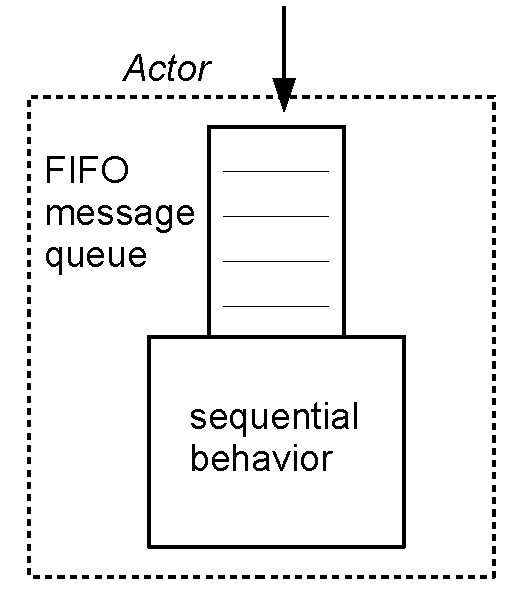
\includegraphics[width=0.4\textwidth]{actor.pdf}
  \caption{Concept of an \textit{Actor} as \\defined by the
          actor model.}
  \label{actor}
  %\vspace{-25mm}
\end{wrapfigure}

The core concepts of the actor model as outlined in \cite{actorsagha}
and \cite{actors2010}
can be summarized as follows. The actor model treats \textit{actors}
(or processes) as its universal primitives of computation.
These actors are autonomous in the sense that each actor's executed
behavior is independent of the concurrent existence of other actors.
However, in order to interact with others, actors can send and receive
messages as illustrated in Fig.\ref{actor}. So each actor consists
of its single threaded behavior and a single input message queue.

The actor can now decide whether or not and how to react to
its incoming messages and can also send messages directly to other
actors. Its behavior itself though is single threaded.
The concurrent nature of an actor based system lies within the
actor model itself because of the actors being executed independent
of each other.

This also means that the only means of communication,
namely message passing, is \textit{asynchronous} by default.
The actor model iself does not define any receipt or acknowledgement mechanism
for messages received by an actors input queue. Any such communication
protocol must be implemented by the actors themselves, e.g. by
programming their behavior to send an acklowdgement to the sender once
a message is processed. This means that, using the plain actor model,
a sender cannot infer whether or not its message was processed
or perceived by its receiver. It cannot even infer whether or not
the message ever reached the receiver.
\newline

This seems ludicrous compared to the implicit safety and messaging
guarantees promised by the \textit{distributed objects} approach
presented in chapter \ref{DistributedObjects} where synchronous
messaging is as \textit{easy} as a local function call. But this
seemingly pessimistic approach to messaging turns out to be
acceptably close that what must be anticipated when dealing with
messaging in highly distributed systems on the data center and cloud
scale.

So again the actor model seems to provide a sweetspot because on
the one hand it encompasses characteristic properties of highly
distributed systems, i.e. virtually no message delivery guarantees,
thereby forcing the developer to deal with these circumstances
\textit{explicitely} in her program structure and application design and on the other
hand provides small, independent and single threaded units of
computation in order to build more abstract and higher level
distributed applications.

\setlength{\intextsep}{10pt}
\setlength{\columnsep}{20pt}

\begin{wrapfigure}{l}{0.5\textwidth}
    \begin{lstlisting}
-module (send_recv).
-compile([export_all]).

serve() ->
  receive
    {Request} ->
      io:format("received request~n"),
      serve()
  end.

run() ->
  Pid = spawn(?MODULE, serve, []),
  Pid ! {Request},
  ok.
    \end{lstlisting}
  \caption{Erlang example of how to spawn an Actor using the \textit{spawn}
          function and how to use the messaging operator \textit{!}}
  \label{erlang-example}
 % \vspace{-20mm}
\end{wrapfigure}

Since Erlang is an actor based language, Fig.\ref{erlang-example}
shows a small example. It spawns an actor executing the
user-defined \textit{serve()} function. Spawning an actor is done
using the built-in \textit{spawn()} function. The serve() function
contains a \textit{receive-loop}, another Erlang built-in indicated
by the \textit{receive} keyword. This loop listens for incoming
messages and tries to match any incoming message to any of the
given patterns. So it can be thought of as the combination of an
implicit event loop and a switch-case statement.

In the case of this example any message that consists of only a single
\texttt{Request} \textit{atom} will be matched to the user-defined
\texttt{Request} \textit{pattern}, triggering
a simple console print and a recursive call to restart the receive
loop. This is important because when the receive loop is entered it
will wait for incoming messages indefinitely unless a timeout is
specified. When a message arrives at the inbox that can be matched
against one of the provided patterns it will be processed as
programmed. When there are multiple messages in the actors inbox
that could be matched against some provided pattern only one
of them is being process and it is up to the actor when to
reenter the receive loop in order to process the remaining messages.
If a message is received that cannot be matched to any pattern, the
message is ignored but kept.
\newline

To address the actor or process created by the call to \textit{spawn()}
a process identifier (PID) is returned by spawn, which is the only
way to attain such an identifier. In order to send messages to this
PID Erlang provides the messaging operator \textit{'!'}.

This shows that message passing is an integral part of the core
language, including its pessimistic delivery guarantees (none), and
specified by the language itself. These semantics are therefor
not loosely defined in some library documentation that could
change any minute but are guaranteed to the programmer,
independent of the language implementation or execution environment.
\newline

Unfortunately there is a down side to this approach. Since the
actor model focusses so heavily on its actors, the result is that
the actual description of the system happens implicitely and
indirectly. It is more like the system \textit{emerges} out of all the
little steps and interactions of its components. To the effect that,
given a running system of maybe a hundred or a thousand actors
\cite{uber}, how would one come to understand what the system is doing
as a whole?

There is no other option than to just pick any actor and start
reading its code. This means one is forced to reverse engineer the
behavior of the entire system from the internal behavior of its parts
which, needless to say, can be quite error prone and introduces
nontrivial cognitive overhead. In other words, there is no way to
take a look at the system from the birds-eye perspective because
most people believe this implies introducing some form of global
state which would be against any of the goals of the actor model
with its asynchronous message passing and independent processes.
\newline

Another problem of the \textit{Actor Model} or any other process
calculus for that matter, is that any actor can possibily communicate
\textit{directly} with any other actor in the entire system at any
given moment in time. This, combined with the fact that almost every
process calculi including the Actor Model is turing-complete,
means that even the simple question whether or not process 1
ever communicates with process 87 becomes undecidable in the general
case. Which makes it almost impossible to predict the consequences
of shutting down a single actor regarding the behavior of the system,
given a large enough system of actors.

\section{Related Work}
\label{relatedwork}

This chapter will present different ideas and projects which have
served as motivation and inspiration not only for the \textit{Drift} language
but for the entire \textit{Drift} project.

First two talks by Rich Hickey will be presented and the relevant
aspects will be extracted. The first talk discusses the necessity
and design of a ``Language of the System'', especially in the
context of highly distributed systems and the second talk
introduces the concepts of \textit{place oriented programming}
and \textit{value oriented programming} with an emphasis on
the importance of immutable data in programming language design.

Then, as a representative of the \textit{functional programming}
approach, \textit{Cuneiform}, a functional scientific workflow language
and \textit{HiWay}, its distributed execution engine
will be introduced. Both of which are being developed here at the
Humboldt University of Berlin at the department of bioinformatics (WBI)
and have served as a major source of inspiration and opposing
concepts.

After that, core concepts of UNIX-like operating system design
and more importantly of the UNIX shell \textit{bash} as one representative
of a typicall UNIX shell are being introduced. Especially a
mapping between the language constructs of the \textit{bash} shell
and core concepts of functional programming languages will be
presented.

Furthermore a new distributed data base project will be introduced
which tries to combine the functional programming concepts of
immutable data and value orientation with the distributed data base
context of data accretion, distributed logging, time series data
and streaming.

Then the source code version control system \textit{git} will
be introduced because it shows how a seemingly stateful system
on the user facing side can be implemented on top of an immutable,
append only file system of objects addressed by hashes of hashes.

At last a talk by Bret Victor will be summarized in which he presents
his idea of \textit{immediate feedback} in the context of programming
and tooling for programming. In this talk he showcases multiple
prototypes which show how to interactively visualize code and how
this could be used to aid the process of developing software.
The most relevant feature presented will be a \textit{time bar}
which allows to interactively go back and forth through past
states of the code and the actively running program.


\subsection{The Language of the System}
\label{LanguageOfTheSystem}

Rich Hickey is most widely known as the creater and
\textit{Benevolent Dictator for Life} (BDFL) \cite{bdfl} of
\textit{Clojure} \cite{clojure2008}, \cite{clojure2010},
\cite{clojure.org}, \cite{clojure-rationale},
a functional programming language and Lisp \cite{lisp86},
\cite{commonlisp90} dialect.
Clojure runs on the Java virtual machine to allow Java and Clojure interop
in order to utilize the extensive collection of already existing
Java libraries.

Clojure is therefor not a \textit{pure} \cite{pure}
functional programming language but should rather be considered a
pragmatist's compromise of having immutable data by default but
allowing for easy I/O and statefulness whenever neededed.

Although Clojure's \textit{front end} (its syntax) looks a lot like
Lisps syntax, which is notorious for its extensive use of
parenthesis, Clojure's \textit{back end} (its implementation)
focusses heavily on very modern features like
\textit{software transactional memory} \cite{stm} and
\textit{persistent data structures} \cite{persistentdatastructures}
aimed at highly concurrent programming.

Hickey himself has been promoting these features as necessary
upgrades to the object oriented view on programming in order to
fully utilize multicore architectures and is an avid
visitor of conferences of programming language design. He therefor has
a considerable collection of talks and lectures in which he explains
his rationale behind his design decisions \cite{hickey-talks},
\cite{hickey-bestof}.
\newline

One of his more relevant talks regarding the work presented here
is called ``The Language of the System''
\footnote{In the context of this talk and for the rest of the work presented
here the word \textit{system} does not mean \textit{low-level} or
\textit{bits and bytes} as in operating system but rather means
the system as a whole as from a bird's-eye view and more as
described by something like systems theory.}
held at \textit{Clojure Con} 2012 \cite{hickey-systemlang},
\cite{clojurecon}.
In it Hickey criticizes what has already been outlined in
chapter \ref{actorModel}, namely that distributed \textit{systems}
today are being built indirectly by programming individual units and
components and then running them simultaneously, hoping that a
distributed system will almost magically emerge but lacking any
description whatsoever of that system as a whole.

\begin{wrapfigure}{r}{0.5\textwidth}

  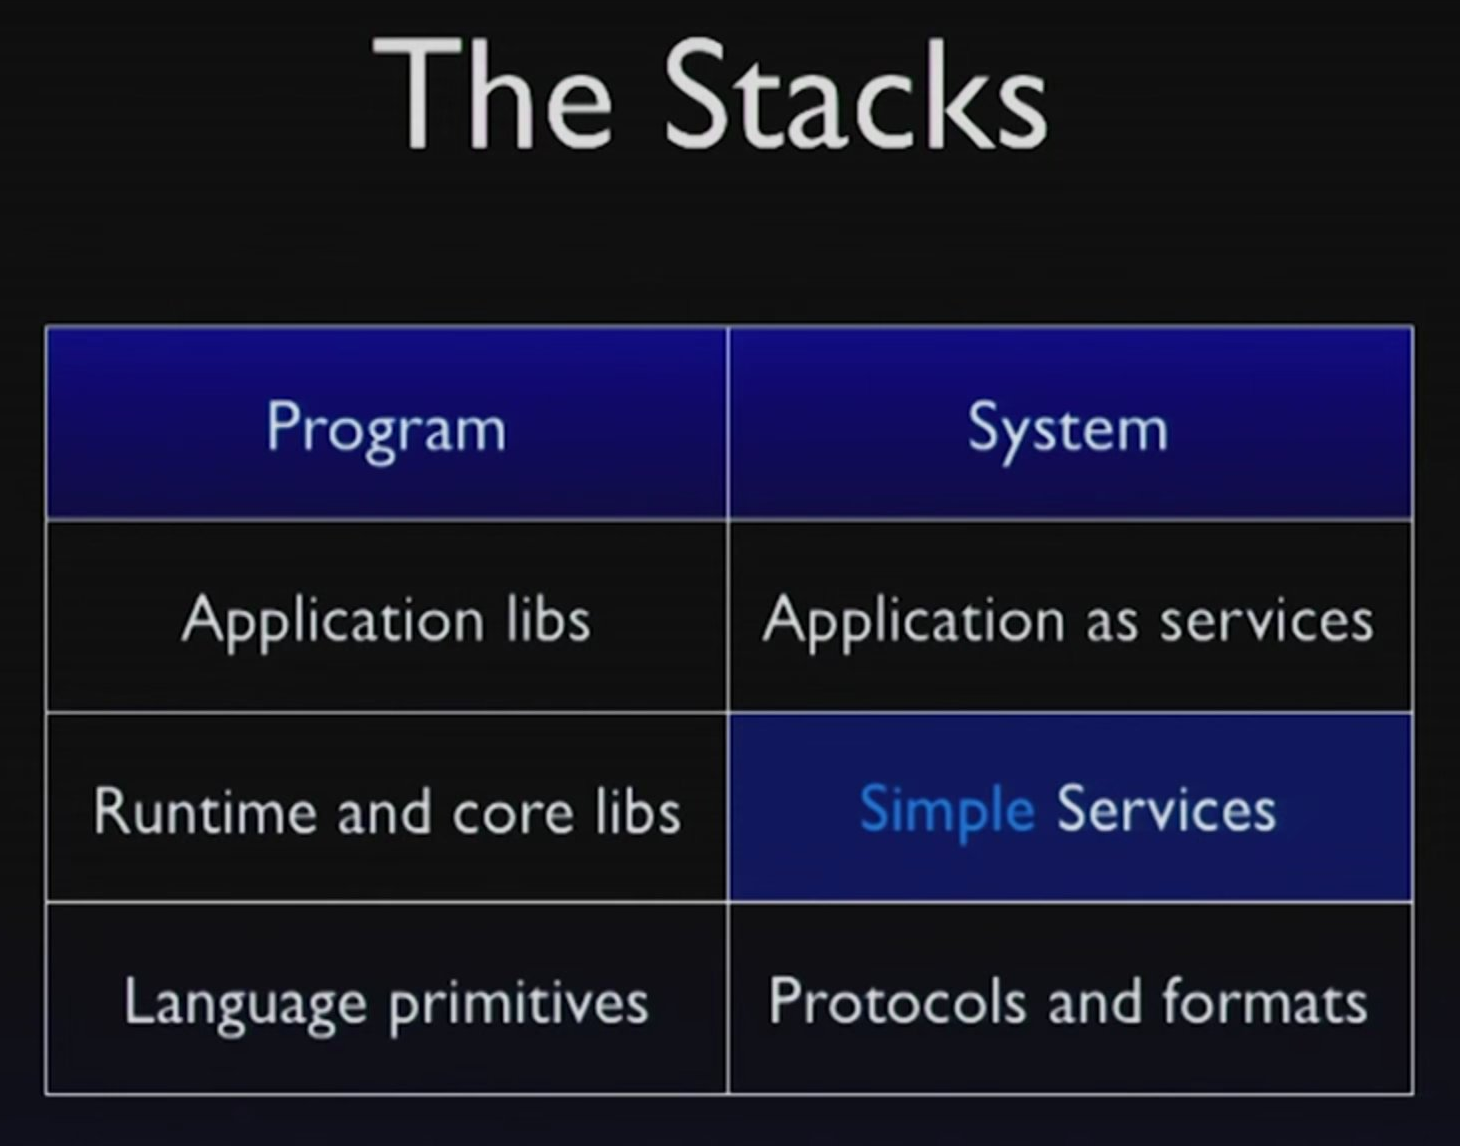
\includegraphics[width=0.5\textwidth]{systemlang.png}
  \caption{Slide-excerp from the talk ``The Language of the System'' by
          Rich Hickey that draws parallels between the composition of
          (local) programs and distributed systems.}
  \label{systemlang}

\end{wrapfigure}

The reason for this, he claims, is that the languages and tools
we use to build each individual component have been developed to
do exactly this: describe \textit{programs}, describe encapsulated
self-contained blocks of computation. They don't provide any
means of describing how to compose these components, because they
don't provide any primitives for how they \textit{communicate}.

As can be seen in Fig.\ref{systemlang} he draws parallels to how
we haven been building our programs in order to derive similar
properties for our system composition and description. For example
he proposes that the language of the system too, would have
primitives just like the programming languages that we have been
using so far. But instead of having primitives of computation like
built-in data types and arithmetic operators, in the systems context
these primitives would be primitives of \textit{communication} like
communication protocols or data formats. On top of which simple
core services need to be available in order to compose higher
level application logic, just like core libraries like
the GNU C library (glibc) \cite{glibc} or any other standard
library of any common programming language provide essential
building blocks for programmers to compose their programs.
\newline

So the relevance of this talk to the work presented here is, that
it sparked the question of whether or not it would be possible to
build such a composition language, a language of the system,
that allowed a global perspective without introducing global
state and how such a language would look like.
\newline

The other talk by Hickey which is relevant to this work and which
I would like to summarize here is called ``The value of values''
and was held at the GOTO Conference 2012 as well as the JaxConf 2012
\cite{vofv-infoq}, \cite{vofv-yt}, \cite{goto2012}, \cite{jax2012}.
Probably being his most famous talk, in it Hickey bootstraps his
views on programming and language design by putting
\textit{immutable data} at the center of programming and deriving
the advantages of core functional programming concepts from that.
He introduces two programming paradigms,
namely \textit{place-oriented programming} and
\textit{value-oriented programming}. A \textit{place} in Hickey's
view literally represents a place in reality. Something where
one can put things and where they reside. If one replaces the thing
that already resides in a place with some other thing, the
information of that exchange is never recorded. Places don't
record their exchange \textit{history} so to speak. Every exchange
\textit{overwrites} the current content of that place.
To the effect that the value received from querying a place
depends on the point in \textit{time} when the query was executed.
The value of the place is inherently intertwined with time, which
is what is generally known as \textit{state}.

This represent the bulk of programming language history. It
even represents the slots on the band of a Turing machine, which
can be overwritten by said Turing machine with symbols defined in
its alphabet. We have built hardware like memory and hard drives
but also our software like data bases and file systems
after this principle. They provide slots of storage which can
carry a value but can be overwritten so the new value replaces the
old and the value received from querying a place depends on the
moment in time of the query.

\begin{wrapfigure}{r}{0.6\textwidth}

  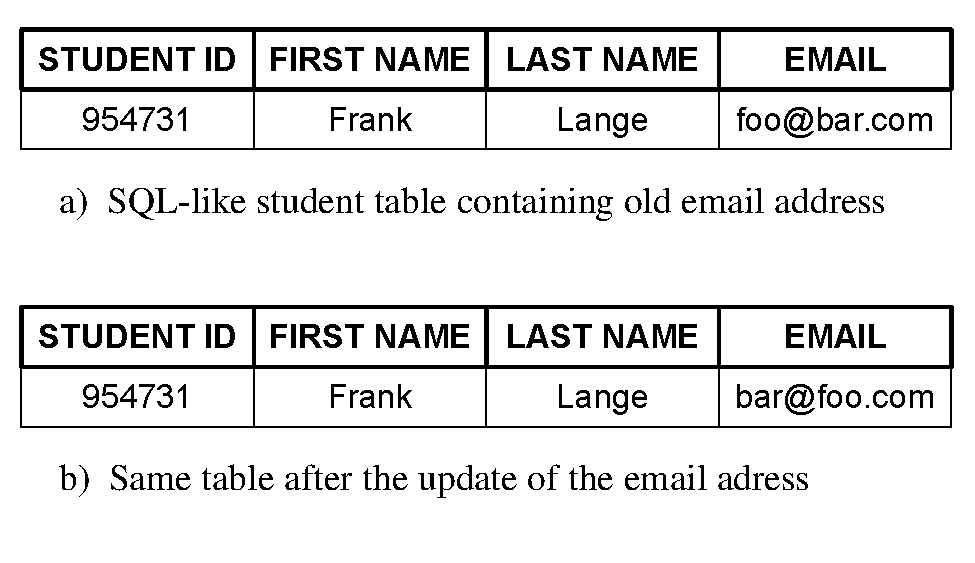
\includegraphics[scale=0.6, keepaspectratio]{sql.pdf}
  \caption{Place-orientation examplified by a SQL table, each cell
           being a place.}
  \label{sql}

\end{wrapfigure}

In order to examplify this concept, Fig.\ref{sql} shows a very
basic representation of what could be a \textit{SQL} table.
This table stores data using the schema of \textit{(ID, First Name,
Last Name, Email)} which is supposed to represent a registered
student. In Hickey's view, each cell of the table is a place, so
if a student were to change her email address only the cell containing
the email address would change, as shown in Fig.\ref{sql}b.
But changing an email address does not invalidate the fact that
there has been a point in time in which the student used the
old email address, just like electing a new president of a country
does not invalidate the fact that the country was once governed by
somebody else.

It is these \textit{facts} that in Hickey's view represent what is also
known as a \textit{value} because a value, once it exists, can never
change. One of the most used and perhaps most accessable examples of
values come from mathematics. The value '5' is just that, five. It
cannot be altered or changed in any way. Five is always five.
Mathematics allows for expressions like \textit{x = 5 + 1} which
binds the expression which uses two values and an operator to
the \textit{name} x. One could now \textit{evaluate} the subexpression
\textit{5 + 1} which would yield another value, namely '6', but that
would not change either the value '5' nor the value '1'. Five is always
five, even when used in compound expressions.

This is exactly what \textit{value-oriented programming} is about.
It treats \textit{data} as values, so data is \textit{immutable}
by default. Since data is immutable this means that it behaves
like facts: once created (once it happened) it stays true forever
and since operations on data can never change that data but only
create new data, it becomes easy to record the history of steps
that led to the creation of data. It's almost like one gets the
history of operations on data for free, once data is immutable
which is the direct opposite of place-oriented programming.
\newline

Both these approaches represent the extreme positions on a spectrum
of language and system design. Unfortunately though, both these
approaches in their basic form share a mutual problem: they don't scale.
Place-oriented systems are very \textit{space efficient} because
places are singletons, they are unique and there is only exactly
\textit{one} of each place. This means that all producers and
consumers or all readers and writers working on a place need to
be mutually excluded from doing so. Access to a place needs to
somehow be coordinated. One example for such coordination are
\textit{mutexes} (also called \textit{locks}). However, this means
that with an increasing number of accesses to a place, the
contention for that place increases and the time spent on coordinating
this access increases, especially if each logical operation needs
access to multiple places in order to complete successfully. So
place oriented systems scale in terms of space but not in terms of
time.

As already outlined, value-oriented systems implement the exact
opposite. Because values can never change, it is absolutely
safe to allow multiple access to a value, or give each accessor
its own copy. To stick with the mathematics example, it is common
to see multiple functions using the value '5' as one of their
input values. One calculating the square of its inputs the other
something completely different. Although both are working with
the same \textit{value} they are working with their own copies of it,
which don't have to updated or coordinated in any way, because
five is always five. The value cannot change. This means that there's
virtually no coordination overhead which allows value-oriented
systems to scale in time, but because multiple instances or copies
of the same value might need to exist, the system does not scale in
space.
\newline

So the choice every language or systems designer needs to make,
is which scalability bottleneck the system will be able to cope with.
Is space going to be the issue, so it is important to be space efficient
and feasible to pay for that efficiency with coordination overhead,
because contention will be sparse? Or is contention going to be the
issue, so that it is easier to supply enough space in order to keep
the coordination overhead to a minimum?

As I would like to argue, in the context of future
distributed systems,
the latter approach seems more appropriate because until now, we
have tried to simply port our place-oriented systems like file
systems and data bases into the distributed context and it didn't
seem to work out all that well. I argue that distributed systems
are not so much about place-efficient computation, but rather about
\textit{communication} and \textit{coordination}. Which means that
a value-oriented system will keep the overhead for these things to
a minimum and it is way easier to supply enough space, than to make
a place-oriented system scale in the distributed context.



\subsection{The Cuneiform Language}
\label{cuneiform}

One area that features a wide variety of custom tailored languages
which allow to describe a possibly distributed system from a
bird's-eye perspective, is the field of \textit{scientific workflows}
\cite{kepler}, \cite{swf-survey}.
Especially in the context of \textit{bioinformatics}, scientific
workflow systems like Kepler \cite{kepler}, Taverna \cite{taverna}
and Pegasus \cite{pegasus2004}, \cite{pegasus2005} have become an
invaluable tool because they allow to utilize distributed systems
in order to cope with the sheer amount of data that's been used and
might also allow for massive gains from parallelization.

One language that is beeing developed here at the Humboldt
Universität zu Berlin, at the department of \textit{Knowledge Management
in Bioinformatics}, is called \textit{Cuneiform}
\cite{cuneiform}, \cite{saasfee}.

Matching the approach advocated by Rich Hickey and as presented in
the chapter \ref{LanguageOfTheSystem}, Cuneiform is a functional
workflow language with a formal foundation in the lambda calculus
\cite{lambdachurch}, \cite{lambda-calc} and with an emphasis on
immutable data. Another key aspect of Cuneiform is its
\textit{foreign function interface} which allows to use already
exisiting bioinformatics tools with any modifications. Most
other scientific workflow systems force users to reimplemented
their desired services using the abstractions given by the framework.

\begin{figure}[h]
    \begin{lstlisting}
deftask untar (<list(File)> : tar(File)) in bash *{
  tar xf $tar
  list=`tar tf $tar`
}*

txt = untar(tar: 'corpus.tar');
csv = wc(txt: txt);
result = groupby(csv: csv);
result;

    \end{lstlisting}
  \caption{A shortened word count example using the functional workflow
           language \textit{Cuneiform}}
  \label{cf-example}
\end{figure}

Fig.\ref{cf-example} shows a shortened and small word count example,
taken directly from Brandt et al. \cite{cuneiform}. First this
example shows how a Cuneiform task is defined using the \textit{deftask}
keyword. The task named \textit{untar} is supposed to deliver the
same functionality as the widely known UNIX tool \textit{tar} and
therefor expects a \textit{file} as
input and returns a \textit{list of files} as output. Showcasing the
foreign function interface capabilities, one can see that it is
specified that the body of this task will actually be written in
\textit{Bash}, the language of the same-named UNIX-like operating
system shell.

The actual workflow description is shown in lines 6-9. Since
Cuneiform uses \textit{lazy evaluation} the first lines 6-8
don't actually trigger any behavior of the system. They only
describe the workflow. Line 9 shows the query syntax of the
system, which will finally trigger the actual execution of the specified
workflow and print its result.

As one can see the results of the called tasks are bound to names
using the \textit{=} operator syntax, which in an imperative language
might be called the \textit{assignment operator}. Since Cuneiform follows
the functional programming paradigm, these name bindings, rather than
being assignments, are later dissolved using textual substitution.

Each name in the example work flow is used by the following task
invocation as an input, therefor creating a zick-zack like pattern
which basically describes a sequential data dependency between these tasks.

This shows that the coordination expressed via Cuneiform describes the
data dependenies and therefor the \textit{data flow} between tasks which
cannot only be a sequential flow, but rather can branch out and join
again in any possible way, describing a \textit{directed acyclic graph}
(DAG).

Since Cuneiform uses lazy evaluation, lines 6--8 build the DAG which
can then be optimized or minimalized when the actual query operator
in line 9 triggers its execution.
\newline

The next chapter will try to show, how these core concepts of a
functional language and its data flow describing qualities can be
mapped or emulated by the language used in the common UNIX shell.

\subsection{The UNIX shell}
\label{bash}
Much can be said about the The UNIX time sharing system
\cite{unix78}, \cite{unixdesign}. It was developed in the early
1970's by Dennis Ritchie and Ken Thompson and featured many
new concepts and abstractions which are still widely used today,
like the file system and its naming and file descriptor concepts,
inter-process communication mechanisms and the command line interface
often referred to as ``the Shell'' \cite{unix78}.

It was also written in a new programming language developed by
Ritchie and Brian Kernighan, called the \textit{C} programming
language \cite{c}. So it delivered exactly what today is missing
in the distributed systems community: a complete stack.

\begin{figure}[h]
  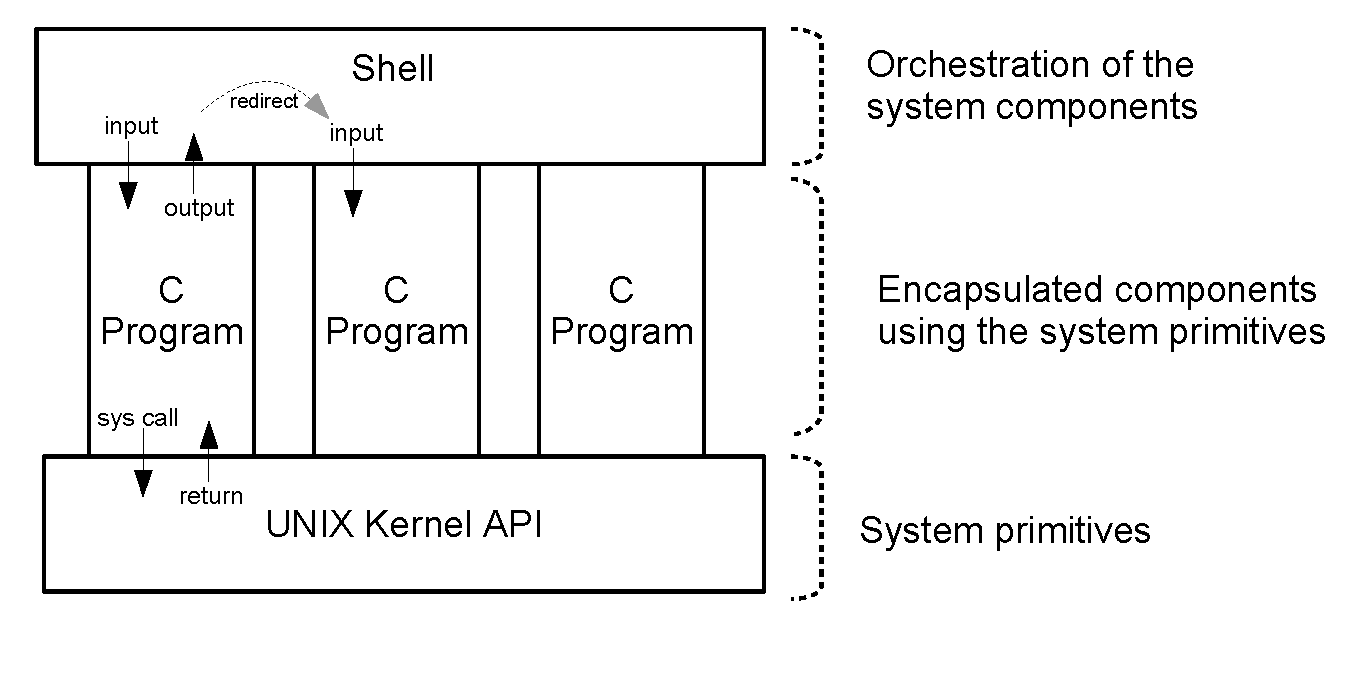
\includegraphics[scale=0.6, keepaspectratio]{unixstack.pdf}
  \caption{Conceptional stack of the original UNIX system}
  \label{unixstack}
\end{figure}

As shown in Fig.\ref{unixstack} the operating system and its
kernel API are positioned at the bottom of the stack. Representing the
foundation by providing basic system primitives in terms of
storage and persistence (memory, file system) but also in terms of
communication (file descriptors, sockets, pipes) although it can be
said that all of these concepts are unified behind an universal channel
concept, namely the file descriptor. Hence the proverb ``In UNIX,
everything is a file''.

The system components are instances of the concept of a \textit{process}.
Encapsulated units of program instances, using virtualized resources like
CPU and memory without any knowledge about other processes and requesting
the system's primitives and services via so called \textit{system calls}.

On top of the stack lies the shell, interfacing with the user.
Using a different language than the system components, its purpose is
to allow the user to control and orchestrate the system by starting
programs (creating a new system component by initiating a new process)
and by either persisting the output of the program to the file system or
chaining subsequent program calls, redirecting the output of one
program to be the input of the next program in the chain
(\textit{pipe mechanism}). Although it is possible for processes
to directly talk to other processes via inter-process communication
mechanisms like \textit{named pipes} or \textit{sockets}, the default
mode of operation is that each process receives its input data from
a designated input channel called \textit{standard in} (stdin) and
can choose between two designated output channels, named
\textit{standard out} (stdout) and \textit{standard error} (stderr),
which direct the output back to the shell who created the process.

This means that each component doesn't know and doesn't have to know
how the whole composition, of which it is being part of, looks like.
It only knows where its inputs come from and where to produce its
output to. In my opinion, this bears much resemblance to the basic
notion of a function and function composition in functional programming.
Also the notion of autonomous processes seem very similar to what
is today known as \textit{Actors} in the \textit{Actor Model},
as introduced in chapter \ref{actorModel}.

\begin{wrapfigure}{l}{0.5\textwidth}

  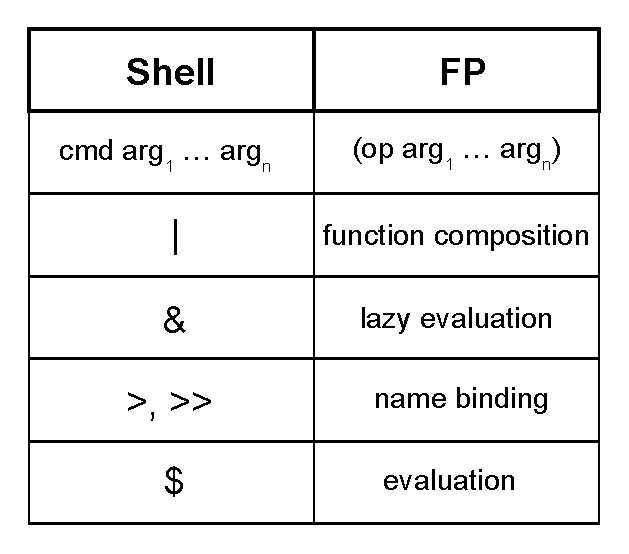
\includegraphics[width=0.5\textwidth]{bash.pdf}
  \caption{Mapping of concepts from the original UNIX shell to
          functional programming concepts.}
  \label{bash}
  \vspace{-100pt}

\end{wrapfigure}

In fact many of the core features and language constructs of a modern
UNIX shell like the \textit{Bourne Again Shell} (bash) \cite{bash}
can be mapped to concepts used in languages following the
functional programming paradigm, as can be seen from the table
shown in Fig.\ref{bash}. First of all the command syntax of the
shell as shown in \cite{unix78} follows the same prefix notation
as used in Lisp \cite{lisp86} with the operator first and the following
space-separated operands, e.g. \texttt{add 3 5} in the UNIX
shell and \texttt{(+ 3 5)} in Lisp.
Another concept is the widely known \textit{pipe operator} \texttt{|}.
This operator redirects the data received from the default output
channels of the program on the left hand side to the default input
channel of the program on the right hand side. In the same way how
function composition in functional languages as well as plain mathematics
\textit{forwards} the result of the inner function as input to the outer
function in an expression like $f \circ g$ which can also be written as
$f(g(x))$. However, the disadvantage of this mathematical notation
is that the data \textit{flows} from the inside to the outside, or
from the right to the left. When using the pipe operator the whole
statement becomes $g\ \textbar \ f$ and the data flows from left to right,
just like most western cultures read any other form of text.

The \textit{ampersand operator} \texttt{\&} signals that the spawned process
should be run in the background. This means that a new shell
prompt is immediately available for the user and new commands can be
entered and processed. Leaving the \texttt{\&}-operator when starting a program
blocks the shell for the duration of running the program and prints its
output to the shell whenever output is made available by the program.
The \texttt{\&}-operator is useful in order to spawn multiple programs but
since no output is shown \footnote{In some implementations the output
is printed whenever it arrives, interleaving with the current user
input} this could be seen as telling the shell
everything that needs to be done before actually querying any results
which is exactly what lazy evaluation does in functional programming
languages.

The single and double angle bracket operators $>$ and $>>$
express that the output of the spawned program shall be redirected into
a file, e.g. \texttt{add\ 3\ 5\ >\ result.txt}. In order to see why this
can be thought of as a name binding one needs to take a closer look
at the concept of a \textit{file system}. Of course, many file
system implementations are highly complex and use different kinds of
strategies and algorithms in order to provide high performance read
and write access to storage hardware like hard drives, tapes or flash
drives. This implementation side of the file system is what I would
like to call the \textit{back end} of a file system and is of less
concern for this matter. However, most
UNIX based file systems share a common \textit{front end} or user
interface which is also defined in \cite{unix78} which uses the notion
of \textit{files} and \textit{directories} in order to create a name tree
and defines the naming scheme of this tree by putting a \texttt{'/'} as its
root and inserting another \texttt{'/'} for every level in the tree. So
a file named \textit{c} which is contained in a directory called \textit{b}
which itself is contained by another directory called \textit{a} would
have the name \texttt{/a/b/c}.
This naming scheme guarantees that each and every file has a single
globally unique name because files are leafs in this name tree and
there is only a single unique path to reach each leaf
\footnote{ignoring more advanced features like symbolic links}.
So from the user perspective, given such a unique name, the file system
fetches the \textit{unstructed} data that is referenced by the name,
which is exactly the user facing behavior of what today is most widely
known as a \textit{key-value store}.
Therefor writing data to a file can be seen as setting the value of
a key in the key-value store but since keys are nothing more than
unique names, this can also be seen as binding the name of the file
to its content, in the same way that a reference points to its data.
\newline
Lastly, the shell features the \texttt{\$}-operator which is mostly used to
query the content of shell variables, e.g. \texttt{echo \$FOO}.
Since the shell interpreter uses \textit{eager evaluation} \cite{eagereval},
i.e. immediately executing each command after its been entered by the
user, it is not possible to put commands into variables and have them
executed only when the content of the variable is querried, e.g.
\texttt{FOO=`cat words.txt | grep dog`}. But following what has earlier
been said about the \texttt{\&}-operator, \textit{if} the
\texttt{\&}-operator can be thought of as lazy evaluation, then the
\texttt{\$}-operator would be the query operator which triggers
command execution. In the same that the \texttt{result;} statement
in line 9 of Fig.\ref{cf-example} querries the result of the described work flow.
\newline

This feature mapping shows, that the basic UNIX shell can be thought
of as a very basic functional language given only minor modifications
and it also challenges the popular belief that imperative languages
and functional languages live on opposite sites of the language
spectrum.

There is however a very fundamental problem with using the UNIX shell,
that is not fixed by interpreting its features as functional and
that is of course its statefulness in regard to the underlying file
system. Since the file system is provided as a system primitive by
the kernel, the shell, being only yet another process running on
the system, has access to the exact same file system as any other
process running on the system. This means that concurrent access
on the same file leads to contention about its content and
is a fundamental problem that needs to be dealt with. Unfortunately
the original design, though aware of the problem,
did not propose any solutions \cite[chapter 3.6]{unix78}:



\blockquote{There are no user-visible locks in the
file system, nor is there any restriction on the number of users
who may have a file open for reading or writing; although it is
possible for the contents of a file to become scrambled when two
users write on it simultaneously, in practice, difficulties do
not arise.}


In that sense, files behave like \textit{places} as introduced in
chapter \ref{LanguageOfTheSystem} but without providing coordination
mechanisms. Since the UNIX shell \textit{language} can easily be
mapped to functional language concepts, it would make sense to convert
the underlying data model from a place-oriented into a
value-oriented one by introducing some sort of an \textit{immutable
file system} in which files are represented as \textit{values} instead of
as places.
Interestingly enough, this idea is currently explored by a new
project coming not from the file systems community but rather
from the data base community, as will be explained in the next
chapter.




\subsection{Datomic}
\label{datomic}

Datomic \cite{datomic} is another project started by Rich Hickey and is now
developed and marketed by \textit{Cognitect Inc} besides Clojure, a Lisp
dialect for the JVM, originally conceived by Hickey, as was introduced in
chapter \ref{LanguageOfTheSystem}.

Instead of being another functional programming language, Datomic
is a distributed data base, delivering classic data base guarantees and
features like ACID transactions, joins and a logical query language.
The main difference however, is that Datomic is based on the
value-oriented idea of immutable data and not based on the idea of
mutable cells in a table (as demonstrated by Fig.\ref{sql} in
chapter \ref{LanguageOfTheSystem}) as explained in
\cite{datomic-architecture} and \cite{datomic-datamodel}.
This is why one of Hickey's talks about Datomic \cite{datomic-talk1},
\cite{datomic-talk2} is called \textit{The Database as a Value}.

As introduced in chapter \ref{LanguageOfTheSystem} Hickey views
data values as facts. Therefor a data base's role of storing data
is nothing more than the accretion of facts, in the same way
that history is an accretion of facts, like ``the king died'' or
``Today I moved to Berlin.'' and even though new facts can be
recorded concerning the same subject or \textit{entity}, these
new facts do \textit{not} invalidate that there was a point in time
in which the old fact was true. New facts do not overwrite old facts.

\begin{figure}[h]
  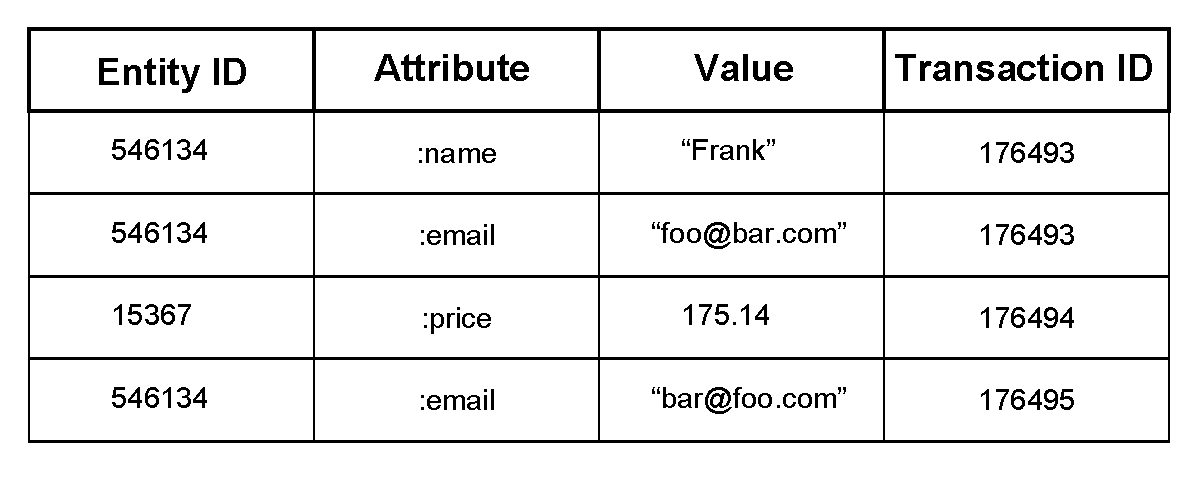
\includegraphics[scale=0.6, keepaspectratio]{datomic_scheme.pdf}
  \caption{The information model schema used in Datomic.}
  \label{datomic_schema}
\end{figure}

So in order to talk about facts at different points in time, Datomic
uses a single schema information model which defines the structure
of every recorded fact. As shown in Fig.\ref{datomic_schema} every
fact is a 4-tuple consisting of an entity ID to uniquely identify
subject for which a new fact is recorded for, the attribute of
the entity for which this is new information, the actual value itself
that we want to record and a transaction ID that serves as a logical
time stamp in order to allow facts to be recorded at different points
in time. The idea of logical time is of course in reference to what is
known as a \textit{Lamport Clock} \cite{lamportclock} and also
\textit{Vector Clocks} \cite{vectorclock1}, \cite{vectorclock2}
and has been used by other distributed storage systems like
Google's \textit{Bigtable} project \cite{bigtable}.

In contrast to the example shown in Fig.\ref{sql} in
chapter \ref{LanguageOfTheSystem} the example shown here in
Fig.\ref{datomic_schema} tries to show how a possible snapshot of
the distributed log of facts might look like in Datomic. As one
can see the first transaction (\#176493) sets two attributes of
the same entity, namely its name and email address. The next
transaction sets the price of some completely different entity
and then another transaction is issued concerning the already
existing entity from the first transaction, recording a new email
address for that entity.

This of course means, that any reader still reading the old
email address won't be interrupted and can still perceive his
outdated view of the world and any new reader can decide whether
he wants to receive the most recent value or the history of a
value. This lends itself to using timed window operations in order
to select only a fraction of the history and brings this system
closer to the field of data streams and event stream processing.




\subsection{Git}
\label{git}

Git is a so called \textit{distributed version control system}
\cite{git}, \cite{gitwiki} created by Linus Torvalds
\cite{gittalk} in order to help the development process of the
Linux operating system kernel, also created by Torvalds.
Since first conceived in 2005 \cite{gitbirth}, \textit{git} has become
one of the most used tools in modern software development today and
very many things can be said about how to effectively \textit{use}
git in order to organize source code versioning
and the whole collaborative software development process \cite{gitbook}.

Unfortunately the information about its internal structure and workings
is disproportionally rare compared to the massive amount of tutorials
and usage guides. However, it is the combination of the internal
structure of git and its user interface that is of relevance to the
work presented here.
\newline

Since git was originally conceived to be a version control system
for source code and source code is most widely stored in files,
git operates on the file level and tracks changes to lines in files.
So from the user perspective, these are normal file system files
which are edited and stored just as any other files. Git does not
interfere with any operations of the underlying file system.
It is therefor completely invisible during the file editing
process.

After a change of a file has been saved (persisted to the underlying
file system) the user can issue git commands, e.g. using the
\texttt{git} command line tool, in order to instruct git to track and
\textit{note} these changes. In order to advance the git repository
to a new state, these changes need to be \textit{commited}. This
will create a new vertex in the history log of git and will advance
the current head pointer of the git repository to this new
version. It's important to note, that there is no fixed commit size.
Commits can contain any number of changes, even of different files.
It is up to the user to decide the \textit{distance} between
steps of progress.

\begin{wrapfigure}{r}{0.5\textwidth}

  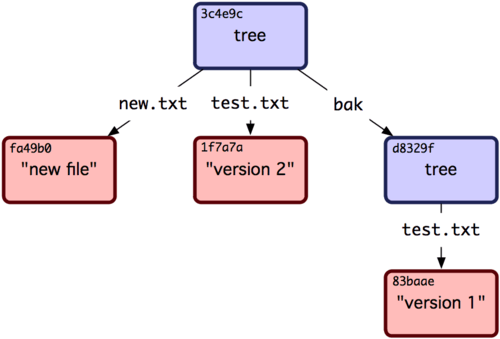
\includegraphics[width=0.5\textwidth]{git.png}
  \caption{Example of Git's internal tree structure based on content hashing.}
  \label{gittree}

\end{wrapfigure}

Git then stores the content of the tracked files as so called
\textit{blobs} and addresses them by the hash of their content.
Therefor behaving like a \textit{content addressable file system}
underneath. In order to store the file and directory structure
a tree structure is used in which blobs represent files and
subtrees represent directories, as shown in Fig.\ref{gittree} which
was taken from \cite{gitinternals}. It's important to note that
if a file is changed by the user and that file is then tracked
and the change committed to git, the hash of the content of the
file will be different compared to the earlier version of the file.
Therefor git will store the complete file again, now with its
new content and under the new hash. Only in later stages of the
repository will git use \textit{delta encoding and compression}
in order to eliminate duplicate content, i.e. when pushing to
a remote repository.
Keeping every single version of file identified by its content
hash is what allows git to be able to go back in time and fully
restore \textit{any} version of the repository ever committed.

This is all completely hidden from the user. From the user
perspective the file that she just changed, really changed.
Because git does not interfere with the underlying file system
a change in a file is persisted and permanent. It's the user
instructing git to take a \textit{content snapshot} of the current
state of the repository containing the content of all its files
and directories when issuing a commit command.

So the content snapshot becomes an immutable \textit{fact} and is
appended to the internal repository history. Just like a fact is
appended to the fact log that is Datomic, as introdudec in chapter
\ref{datomic}. But since the file really changes for the user,
she always immediately sees the latest state of the world but
has the possibility to check out earlier versions of the world.

Therefor the user interface is stateful. If a file is deleted
it's gone from the directory. But it is possible to recreate
the directory state in which it existed, including its content,
if a snapshot of that state was recorded. This means that it is
possible to change a file and then revert the change or to
create a file and then delete it again without git
ever noticing. The user has full control of the
history of the repository and needs to decide which intermediate
states of the repository become immutable facts by instructing
git to take a content snapshot. But since the changing of the
current files and also the recreation of earlier versions happen in
the extact same directory, the user experience feels more like working
in a stateful environment and persisting the current \textit{state}
down to the immutability layer. It feels like a stateful system
on top of an immutable system, instead of just dumping backups to
a data base.
\newline
So it is not necessary to stick to immutability all the way up
to the user interface in order to benefit from the advantages
of an immutable system because user actions aren't always final.
They don't always represent irreversible facts that should always
stay true. As I would like to argue, most people iterate when
working. They have an idea that seems plausible, implement that
idea and then realize that they haven't thought of this and that,
or something else doesn't work out as planned. So they change,
adjust and iterate until a satisfying solution is found or the
necessary resources for doing so have run out. Which is exactly
what is best represented by a stateful environment.

But there will be intermediate steps that seem significant, and
these can be recorded as immutable facts in order to allow for backtracking
or to serve as documentation or as cached results for other work in progress
that somehow arrives at the same intermediate result.




\subsection{Immediate Feedback}
\label{bretvictor}

After having introduced the notion of immutablity and its advantages
in systems design but also the necessity of state and
where it can be a viable tool, the last piece that is needed in order
to introduce the \textit{Drift} project is how to interface with
the user.
As introduced in chapter \ref{cuneiform}, scientific workflow
languages and systems deal with the need of the user to compose
complex work flows from individual parts while maintaining a
bird's-eye perspective on the whole system and for instance there
a number of graphical work flow description languages like

\section{Drift}
\label{drift}

The last chapter, chapter \ref{relatedwork}, introduced multiple
seemingly unrelated software projects and also the people behind
them and their ideas and principles. However unrelated these projects seem,
they each contribute to the work presented in the following
chapters, namely the \textit{Drift} project.

The first idea that was introduced in chapter \ref{LanguageOfTheSystem}
was the need for a language of the system. A language that would allow
to orchestrate a possibly distributed or even microservice based system
from a bird's-eye perspective. In order to allow such a system's
perspective without depending on global state in a distributed
context and to keep the complexity arising from the combinatorial
explosion of contending and interleaving interactions of the
autonomous and independent components of the system to a minimum,
the importance of immutable data in the form of value-oriented
programming was introduced.

Chapter \ref{cuneiform} showed a modern contender for such a
language and system, namely Cuneiform: a functional scientific
workflow language, utilizing most of the functional language
toolbox like lazy-evaluation, single-assign name bindings and
independent subexpression evaluation as defined by the
Church-Rosser Theorem \cite{churchrosser}, \cite{churchrosserwiki}.
However, using Cuneiform and similar systems means fully accepting
the paradigm of functional programming and abandoning any
imperative roots of programming, which seems rather radical given
the wide adoption of imperative languages which shaped the
way people think about programming for generations.

In order to look for alternatives, chapter \ref{bash} went back
in time and took a closer look at a system that has already been
around for decades, namely the UNIX operating system. The interesting
aspect when it comes to system orchestration and coordination from
a bird's-eye perspective is of course the UNIX shell. Given
that the operating system allows for multiple independent
processes to run seemingly autonomous, the shell not only provides
mechanisms to spawn these processes but also to connect
the data flow between them using well-known abstractions like pipes
and files. Furthermore, the chapter \ref{bash} showed, that when taken
seriously, the constructs offered by the shell language can even
be mapped to functional language concepts as used by languages
like Cuneiform. This revealed that the UNIX shell offers roughly
the same capabilities in terms of orchestrating a system of
independent processes \textit{plus} being imperative, widely-known
and interactive.

Especially the interactiveness delivering immediate feedback is
something that provides multiple benefits as was introduced in chapter
\ref{bretvictor} and was something that for the longest time was second
nature in the realm of functional but not imperative programming.

The ``big problem'' so to speak, when it comes to the design of the
UNIX shell as well as the operating system itself and the idea of
porting it to the context of distributed systems is of course the
file system or more generally the data layer. Since its design
follows the place-oriented paradigm as introduced in chapter
\ref{LanguageOfTheSystem}, any subsequent implementations
using distributed file systems have stuck to the same paradigm
and therefor run into the same issues.

So in the same way that chapters \ref{cuneiform} and \ref{bash}
are supposed to challenge the widely accepted believe of
incompatiblity between functional and imperative language concepts,
chapters \ref{datomic} and \ref{git} try to challenge the
preconceptions of distributed immutable data systems and their
implications. So chapter \ref{datomic} introduces Datomic,
a distributed immutable facts log when viewed from the user
perspective, but when looked at from the implementation perspective,
Datomic only creates the illusion of immutability by putting a thin
immutability layer on top of widely-known and already existing
mutable distributed storage solutions. Git on the other hand,
as introduced in chapter \ref{git}, is the complete opposite. It
provides the user with a mutable and stateful perspective on her
own file system built on top of an immutable content addressable
file system underneath.

This again challenges the widespread believe that immutability
or statefulness are system design primitives that define the
system to its core and must be applied throughout the whole system
stack, up to the user interface.
\newline

So naturally the challenge arose, of whether or not it would be
possible to build an imperative and distributed
shell language with a flat learning curve using well known
imperative concepts  but with the same orchestrational powers and
interactiveness as provided by functional languages on top of
an immutable distributed file system in order to utilize the
benefits of the value-oriented approach and to keep the contention
and complexity of the whole system to a minimum.
\newline

The following chapters will present the current result of that challenge
by first introducing the \textit{Drift language}, a tiny and abstract
microservice coordination language built on the concepts of names,
namespaces and services. Then its distributed implementation including
the immutable \textit{Drift file system} will be presented, which
provides the illusion of a file system by utilizing distributed
message queues. Finally the \textit{Drift UI} will be presented
which is implemented as a web interface for any modern browser
and contains not only the shell but also a visual live-representation
of the system state using the well known Petri Net syntax as well as
a time bar that allows to revisit old system states.



\subsection{The Importance of Names}
\label{importanceofnames}

Developing a programming language can be an overwhelmingly
ambitious task. Most often it's only that when one sets out
to do so, that one realizes how many features even
basic languages offer: arithmetic, different types of loops,
conditionals, logical operators, built-in data types and a
type system that allows for arbitrary user-defined types.
Depending on the overall paradigm the list might continue
with things like classes, objects, inheritance, polymorphism
and generic types or things like type classes, higher-order
functions, partial application or monads and do-notation.

Although it would have been nice to have at least scratched on
some of these aspects, it became clear right at the beginning
that most of these features would be left untouched given the
scope and resources of the work presented here.

But that is not necessarily a bad thing. Constraints often times
have the benefit that they force resources to be spent on what
really matters and so in that same spirit the goal for the
Drift coordination language was to carve out what is
\textit{essential} to programming. It could almost be said that
the goal was to find the smallest possible language that
would not allow for any construct to be taken out and still be
offering the same possibilities.
\newline

So what is the essence of programming?

Well that depends on what the user is supposed to be able to express
in that language. If it's computation through calculation, built-in
arithmetic operators like $+$ or $*$ might seem a good idea. If
the user should be able to express things that model the real world,
like in many simulation contexts for example, having constructs
that represent real world objects and allow for equipping them with
properties like color or weight could be another sensible approach,
built on basic arithmetic. This would naturally lead to built-in
data types for which these basic arithmetic operators are
defined and would build up to a type system which could deal with
arbitrary user-defined types and the operations defined on them.

But defining these structures, functions or classes and modelling their
properties and functionalities is only one part of constructing
a program because these structures in and by themselves have nothing
on which they could execute their behavior on and are not connected
in any way in order to produce a final output as the result of
multiple functionalities chained together.

A program does not only exist as the mere sum of its parts but
also of a description of how these parts interact and compose and
where data comes from and where it goes which is what is mostly
described inside the \textit{main-method} which virtually
all programming languages independent of their paradigm have in
common because it serves as the universal starting point of a program.

Most languages use the same syntax and semantics
for both purposes: for describing the individual components and for
describing their often times more abstract orchestration.
This is demonstrated by the examples shown in Fig.\ref{c-and-java}.

\begin{figure}[h!]
    \vspace{5mm}
    \begin{subfigure}[b]{0.41\textwidth}

    \begin{lstlisting}
#include <stdio.h>

struct point {
  int x;
  int y;
};

int point_sum(struct point p) {
  return (p.x + p.y);
}

int main() {

  struct point p;
  p.x = 3;
  p.y = 5;

  printf("%d\n", point_sum(p));

  return 0;
}
    \end{lstlisting}

      \caption{Component definition and orchestration in C.}
      \label{fig:c-example}
    \end{subfigure}
    \hfill
    \vspace{10pt}
    \begin{subfigure}[b]{0.54\textwidth}

    \begin{lstlisting}
public class Point {
  private int x;
  private int y;

  public Point(int x, int y) {
    this.x = x;
    this.y = y;
  }

  public int getSum() {
    return (this.x + this.y);
  }

  public static void main(String[] args){

    Point p = new Point(3, 5);
    System.out.println(p.getSum());

    return;
  }
}
    \end{lstlisting}

      \caption{Component definition and orchestration in Java.}
      \label{fig:java-example}
    \end{subfigure}

  \caption{Examples of component definition and orchestration done in
           languages that use the same language for both tasks.}
  \label{c-and-java}

\end{figure}

The left hand side figure, Fig.\ref{c-and-java}a, shows an example
using the C programming language. In it, a new compound user-defined
data type \textit{point} is declared and defined, consisting of two
integers representing the x and y coordinates of a point.
Then a function is declared and defined which takes such a point
as an input and returns the sum of its coordinates.

These are the blue prints of the components of this tiny system.
Inside the main-methode an \textit{instance} of a point is created and
its coordinates are set to the values 3 and 5, which are part of
the source code itself. Then a function call is issued using a copy of
this point instance which creates a single instance of the mentionend
function whose return value is then immediately printed to the screen.

So inside the main method the actual \textit{business logic} of
the program is described by composing and chaining instances of the
described components and inserting data into the system and letting
it flow through the components in order to produce the desired output.
\newline

The same thing happens in the example on the right hand side, in
Fig.\ref{c-and-java}b, this time using the object oriented
programming language Java. In this example a class \textit{Point} is
defined, also using two integers to represent its coordinates.
The class defines two methods: a constructor method for ease of
instantiation and a \textit{getSum(int, int)} method to again
calculate the sum of the coordinates.

As with the C example on the left, this plain class definition
by itself would not make for much of a program. The business logic
is again defined in the main-method, where an instance of the Point
class, a Point object, is instantiated (again with data contained
inside the source code file itself) and the result of a call to
its instance method \textit{getSum} is printed.
\newline

However, it is possible to disentangle the component description
from the higher level component composition. One example of this
has already been introduced, namely the UNIX stack as shown in
Fig.\ref{unixstack}. In this stack, each component is a UNIX
process, dealing only with the task of processing the data its
been given and producing its output respectively. The higher-level
business logic of the system is then defined using the shell
which can be used to instantiate components (processes),
just like objects are instantiated in Java, and describe the data
flow between them. The difference is, that the shell language, the
\textit{coordination language} is completely
different compared to the \textit{computation language} used to
describe the computation done by each individual process.

So which of the two, computation or coordination, is actually
more relevant in the context of programming a distributed system?
Well, how would one distribute a computation like $1 + 2$?
Computation in and by itself has something local about it because
the operator needs to have perceived or received its operands in
order to carry out its computation. The \textit{distributedness}
actually emerges because although each individual operation is
carried out on a local machine, the actuall composition of multiple
operations and data flow through them spans multiple locations, i.e.
multiple machines.

So as I have already tried to argue in chapter \ref{LanguageEvolution},
for the context of distributed systems, it's not so much computation
that defines the programming of distributed systems (because
of computation having this inherently local aspect to it, we
can for the most part reuse the already existing computation languages)
but rather \textit{coordination} and \textit{communication} between
the components and operations residing on different machines.
\newline

So the question of what is the essence of programming
changes in the context of distributed systems and therefor for the
context of this work to: what is the essence of composition?
\newline

To me, as far as I can work out, the essence of composition
is simply \textit{data} and \textit{functionality}. Whether
functionality is provided by plain functions modelled after
the example of mathematical functions, or with objects that
encapsulate functionality via methods, or with actors or
processes or microservices is not really important.

I believe the user needs these two things: she needs to be
able to identify and talk about her data and she needs to be
able to identify and invoke her services with that data.
This also includes identifying the data that might be the
result of such a service invocation.

So what's the most natural way for \textit{people} to identify things?
By giving them \textit{names}. Names that carry \textit{meaning}
and therefor provide semantics (for humans).
\newline

\textit{Meaning} is an interesting word and one can easily find examples
where it is ascribed to mechanisms that do not really provide it.
For example one of the fundamental books on programming language
semantics and type systems, \textit{Types and Programming Languages}
by Pierce \cite{pierce} contains the following quote by Mark Manasse
on page 208:

\begin{quote}
The fundamental problem addressed by a type theory is to ensure
that programs have meaning. The fundamental problem caused by a
type theory is that meaningful programs may not have meanings ascribed
to them. The quest for richer type systems results from this tension.
\end{quote}

In this quote, type systems are identified as the source of
meaning for programs and there is some truth to that. But I
would like to argue that it is not the type system itself that
provides the meaning, but rather the \textit{names} of the types
that do so.
\newpage

\begin{wrapfigure}{l}{0.54\textwidth}
  \begin{lstlisting}
void runServer(ServerSocket serverSock) {
  serverSock.listenOnPort(9000);
}
  \end{lstlisting}


  \begin{lstlisting}
void runServer(Uhjgj abcdeg) {
  abcdeg.inufdhg(9000);
}
  \end{lstlisting}

  \begin{lstlisting}
void runServer(143 abcdeg) {
  abcdeg.inufdhg(9000);
}
  \end{lstlisting}
  \caption{Example showing the importance of \textit{names} for
           human understanding and reasoning about code.}
  \label{type-names}
\end{wrapfigure}

Consider for example the three versions of the same function in
Fig.\ref{type-names}. The first version represents the kind of
code that is used in software development today, using meaningful
names not only for the data types but for the variable names as well.
This makes it easy for humans to understand why a server socket
has a method that triggers listening on a port and why this method
receives a number as input. Most of the meaning is conveyed through
the names, if chosen appropriately.

In the second version the names are obfuscated but still used as
expected by the compiler. This will happily compile, but most of its
meaning is gone. The third version reduces the type identifier to
a number. Most language grammars do not allow for type names to
be numbers, so this won't compile but the type checking engine itself
would probably still accept it. Because to the type checker, the type
is just an ID and as along as it can check whether or not the type
with the ID 143 provides a method with the used identifier and
signature, it would not raise any flags.
\newline

The \textit{meaning} is not conveyed by types. It's conveyed
by the \textit{names} of the types and of course the names of
variables, methods, classes, objects, and so on.
\newline

\begin{wrapfigure}{l}{0.4\textwidth}
  \begin{lstlisting}
int add_one(int n) {
  return (n - 1);
}
  \end{lstlisting}
  \caption{Example showing a bug that cannot be detected by
           the compiler or type checker.}
  \label{add-one}
\end{wrapfigure}

Consider another example, shown in Fig.\ref{add-one}. This example
shows a simple function whose name suggests that it returns its
argument incremented by one. Unfortunately its code does the exact
opposite and returns the decremented input. This will also
happily compile because \textit{add\_one} is a valid function identifier
and \textit{n - 1} is a valid operation on integers. But we as people
will immediate spot the mismatch between the meaning of its name and
its provided functionality.

So when one tries to reduce coordination down to its core parts,
namely data and services, the essential abstract thoughts that can
be expressed by the programmer are something like ``do this on that'',
or ``do this on that and put the result there'', or ``do this
on that and then that and put the final result over there''.
Interestingly even on such an abstract and rather comical scale,
these abstract statements can be categorized into two groups.
They are either describing a functionality chain, where each
component depends on the output of its predecessor and they
all form a sort of pipeline through which the data flows
sequentially or the services are completely independent of
one another.

So naturally the formulation of data and services forms a
dependency tree or, depending on the allowed complexity,
a directed acyclic graph (DAG). Which can be used effectively
for visualizations as will be shown in later chapters.

\subsection{The Drift Language}
\label{driftlang}

And so, in that same spirit, the basic concepts of the \textit{Drift}
language are \textit{names} to represent data and \textit{services}
to represent functionality.

\begin{figure}[h]
    \centering
    \begin{subfigure}[b]{0.4\textwidth}

  \begin{lstlisting}
.> Cat mydata
Lorem ipsum dolor sit amet,
consectetur adipiscing elit.
.>
  \end{lstlisting}

        \caption{Simple service invocation.}
        \label{cat1}
    \end{subfigure}
    \hspace{20pt} %add desired spacing between images, e. g. ~, \quad, \qquad, \hfill etc.
      %(or a blank line to force the subfigure onto a new line)
    \begin{subfigure}[b]{0.4\textwidth}

  \begin{lstlisting}
.> myresult = Cat mydata
.>
  \end{lstlisting}

        \caption{Service invocation with result bound to a name.}
        \label{cat2}
    \end{subfigure}
    \caption{Basic service invocation mechanism in Drift.}\label{drift-examples1}
\end{figure}

Fig.\ref{drift-examples1} shows the basic concepts offered by
the \textit{Drift language} as implemented by the \textit{Drift shell}.
In the Drift language, service names are required to
start with an upper case letter, whereas names representing
data are to be started with a lower case letter. The \texttt{.>} symbolizes
the shell prompt. The first example of Fig.\ref{cat1}
shows the most basic use case: a simple service invocation.
Following the tradition of the UNIX shell, Drift uses the same
order of command and arguments, namely
$Service\ name_{1}\ ...\ name_{n}$.
Depending on the called service it would also be possible to
invoke services without any parameter names.

Since Drift is eager-evaluated the service shown in
Fig.\ref{cat1} is immediately started. In this case it's
a service called \textit{Cat} in reference to the widely-known
UNIX tool, which prints the content of given files to the screen.
So the \textit{Cat} service also returns the data of its arguments and
since there are only names in Drift, the \textit{Cat} services takes names
as input and returns the data associated with them.

Since the data returned by the invocation of the \textit{Cat} service is
not bound to any name, it just gets printed to the shell. When all
the data that is available behind the name(s) given to \textit{Cat} has been
printed, a new shell prompt is shown and further commands can be entered
by the user.

Fig.\ref{cat2} shows the same service invocation but this time the
result of the service call is bound to a name, using the assignment
syntax as known from other imperative languages. Again the
\textit{Cat} service is invoked immediately but since its result
is bound to a name, nothing is printed to the screen except a new
prompt so that new commands can be entered.

\begin{figure}[h]
    \centering
    \begin{subfigure}[b]{0.4\textwidth}

  \begin{lstlisting}
.> myresult = Cat mydata
.> $myresult
Lorem ipsum dolor sit amet,
consectetur adipiscing elit.
.>
  \end{lstlisting}

        \caption{Using the \$-operator to query the data behind a name.}
        \label{cat3}
    \end{subfigure}
    \hspace{20pt} %add desired spacing between images, e. g. ~, \quad, \qquad, \hfill etc.
      %(or a blank line to force the subfigure onto a new line)
    \begin{subfigure}[b]{0.4\textwidth}

  \begin{lstlisting}
.> Cat mydata
Lorem ipsum dolor sit amet,
[cancel]
.>
  \end{lstlisting}

        \caption{Canceling an ongoing data query.\\}
        \label{cat4}
    \end{subfigure}
    \caption{Basic query and query cancelation mechanism in Drift.}\label{drift-examples2}
\end{figure}

In order to query the data that is represented by a name, Drift offers
the \$-operator, a designated query operator, as shown in \ref{cat3}.
This query operator will receive \textit{all} the data available
behind a name and print it straight to the screen.

However, since services are invoked immediately and therefor executed
immediately, it is possible that the service has not yet produced
a single data item or has not yet finished processing and has
therefor not finished producing all of its output. This means that
it is absolutely possible that either no data or only some data is
shown, depending on what's available when the user issues the query.
\newline
Drift is not an \textit{all or nothing} batch system where the user
either sees no output, or all the output atomically. It's a streaming
system in which data is observable whenever it is available. This is
based on the observation that batch processing, even distributed
batch processing, is only \textit{a special case} of stream processing
and not the other way around, as was also proclaimed in
\cite[chapter 1]{flink}. This fits perfectly with the overall
approach of immediate feedback because not only the commands of
the shell are eagerly evaluated and because of that the services
immediately spawned, but also the data produced by the individual
components flowing through the system can be immediately observed
by the user.
\newline
Of course it would defeat the purpose and reactiveness of the system
if the user would have to wait for all the data to be finished, once
querying a name. Therefor query cancelation has been implemented as
shown in Fig.\ref{cat4}. When data is printed to the screen, either
because the result of the producing service invocation was not bound
to a name, or because a name was queried using the \$-operator, the
display of data can be canceled simply by pressing $q$ and new prompt
will be shown so that new actions can be taken.

Therefor printing data to the screen has not the role of presenting
real results, like in many batch processing systems. It rather becomes
a tool for the user to sneak a peek at what the system is currently
doing in order to assess whether or not the system is working
towards the desired result.
\newline

So where do all the available services and names come from?
In the same way that the UNIX shell does not provide much
built-in functionality except for only a very few built-in
commands, the Drift shell also does not provide any services.
Services need to be inserted into a \textit{service registry}.

This is a designated service invisible to the user that the
Drift shell assumes to be available at all times. When a command
is entered, the shell will consult the service registry about
whether the service exists and whether its usage corresponds to
its specification stored in the service registry.

However the shell does not \textit{download} the required service
in any way. It only fact-checks the service before issuing the
entered command as a task to the back-end system, as will be
described in chapter \ref{driftimplementation}.
If a service is unknown to the service registry, a
\textit{service unknown} error will be printed to the screen
and a new prompt is shown.
\newline

The availability of names is different. One of the design goals
of the Drift shell is to present the user with its own cloud so
to speak. Therefor any Drift shell invocation starts a new
\textit{session} using a UUID as a unique session identifier.
In the current implementation, this UUID is also generated and
handed out by the service registry.

Following this principle, any session starts with a
completely empty \textit{namespace} containing no names. However,
before the actual session starts and the entering of commands is allowed,
the user is presented with a setup phase. In this \textit{import phase}
she can only use the \textit{import} keyword to \textit{upload}
files from the local file system, of whereever the Drift shell is currently
running on, into the Drift system.

When the user has finished the import phase, the actual session
begins and normal command input is possible. The \textit{import}
keyword and therefor any further imports are disabled.

\begin{wrapfigure}{l}{0.35\textwidth}
  \begin{lstlisting}
Session: e3d78ad5-898...
.> import data.csv
.> import test.txt
.> q
-------------------
.> ls
  data.csv
  test.txt
.> result = Cat test.txt
.> ls
  data.csv
  result
  test.txt
.> export result as result
.> q

  \end{lstlisting}
  \caption{Example of a short Drift session.}
  \label{drift-import}
\end{wrapfigure}

Fig. \ref{drift-import} shows an example session including the import
phase. Here two local files, namely \texttt{data.csv} and
\texttt{test.txt} are uploaded to the Drift back-end. When the
import phase is finished by pressing $q$, the normal session
begins. This example also introduces one of the few built-in
commands of the Drift shell, namely \texttt{ls}. These built-ins
are again lent from the original UNIX shell and UNIX file system,
so \texttt{ls} is of course used to list all the available names
in the current namespace.

Now with these imported names and associated data, services can
be invoked and their result can be bound to new names. In order
to recognize whether a name resulted from an import or was later
created during the session, only the imported names are allowed
to contain dots and file endings like \texttt{.txt}, \texttt{.csv}
or \texttt{.tar}.

In the same way that the import keyword during the import phase
allows to fill the initial namespace with names, the \textit{export}
keyword allows to \textit{download} the data referenced by a name
to the local file system under a given name. In the current
implementation this can be done at any time during a session
but it could also be a valid alternative to put the export
behavior into a seperate export phase before closing the session.

The local file in which the data is stored is placed inside a
directory with the same name as the session ID, eliminating the
possibility of name clashing between different sessions (of
possibly different users). However, the user of a session is
responsible for preventing name clashes from within a session
when using the \textit{export} keyword.
\newline

So far \textit{names} and \textit{services} and their basic
usage have been introduced. Initial data can be uploaded from
the local file system into the Drift back-end and imported as
names into the initial name space of a session of the Drift shell.
Resulting data from service invocations can be either printed
to the screen or bound to names using the assignment syntax known
from other languages and the namespace can be explored by using
well known UNIX file system commands like \texttt{ls}.

However, there are services whose result is not just singular data.
As has already been mentioned, one possible file extension for
imports is \texttt{.tar} and so naturally one service which is
able to deal with such imports is called \texttt{Untar*},
with the \texttt{*} on the right hand side being of significance
because it indicates that the output of \texttt{Untar*} is not
just data (a single file) but rather a bunch of names.
Which is why the concept of \textit{names} in the Drift language
is expanded to also include \textit{namespaces}, which directly
correspond to directories in the original UNIX file system.

Since the result of an invocation of \texttt{Untar*} is a
namespace, it wouldn't really make sense to be able to print
it to the screen. But it would also not make sense to bind
a bunch of names to only a single name, as was shown so far.

Therefor, the result of services returning a namespace must
also always be bound to a namespace.

\begin{wrapfigure}{l}{0.4\textwidth}
  \begin{lstlisting}
Session: e3d78ad5-898...
.> import comments.tar
.> q
-------------------
.> ls
  comments.tar
.> res/ = Untar* comments.tar
.> ls
  comments.tar
  res/
.> cd res/
.> ls
  c1
  c2
  \end{lstlisting}
  \caption{Example of a name space binding.}
  \label{untar}
\end{wrapfigure}

As shown in Fig.\ref{untar} \textit{namespaces} also start with
a lower case letter, just like names but namespaces must always
be trailed by a \texttt{/}. This and the additional \texttt{*}
allow the interpreter to syntactically verify that the issued
command is at least valid in terms of its basic format.
If the format is invalid an error is printed to the screen to
inform the user and the command is not accepted.

The resulting namespace then of course contains the unpacked
files as new names. This allows the namespace of the whole session
to become a namespace tree in the same way that the UNIX file system
offers a naming tree, with \texttt{/} as a delimiter. Using another
shell built-in, \texttt{cd}, the user can also \textit{walk} the
namespace tree just as with the usual UNIX file system, as is
also demonstrated in the example shown in Fig.\ref{untar}.

This is important because since there are no variables in the
Drift language, only names and namespaces one could now say
that either the original file system was liftet up into the
language or the language allows its variable-space to be
traversable like a tree. Both interpretations are valid.

But not only the variable-space or data-space forms a tree. As
was already mentioned, also the orchestration of services and
the data flow between them forms a tree or possibly even a DAG.

In order to allow for such composition, the Drift language also
features the \texttt{|}-operator (pipe operator) which behaves
exactly like the pipe operator already known from the UNIX shell
as introduced in chapter \ref{bash}. Fig.\ref{pipe-example}
shows one possible use of the pipe operator in order to
count the number of lines of comments that might have been
left under an online video or blog post.

This again showcases the \texttt{*} syntax, which is not only
needed in order to indicate that a service \textit{produces}
a namespace but also to indicate that a service \textit{receives}
 a namespace as input. Therefor the interpreter can immediately check,
(with help of the service registry)
whether or not the basic formats of names, namespaces and services
are valid. But this is not only supposed to help the interpreter.
It is of course done with the best intentions for the user, so that he,
given meaningful names and these basic format identifiers, might
intuitively understand even longer chains.

\begin{figure}[h]
    \begin{lstlisting}
Session: e3d78ad5-898...
.> import comments.tar
.> q
-------------------
.> linesOfComments = Untar* comments.tar | *Concat | LineCount
.> $linesOfComments
  4653
.>
    \end{lstlisting}
  \caption{Example of using the pipe operator and \texttt{*} syntax.}
  \label{pipe-example}
\end{figure}

However, it is not
immediately obvious why such an operator is actually needed.
As was shown so far, the result of every single service invocation,
whether it returns singular data or a namespace, could be bound to
a name or namespace respectively. Leaving it at that, would create
the same zick-zack pattern as demonstrated in Fig.\ref{cf-example}
in chapter \ref{cuneiform}. Unfortunately this would lead the user
into a direction that is opposite to the core philosophy of the
Drift language.

In Drift, there are only names. Not because this makes things
easy but rather because it is the \textit{names} that carry all
the semantics for us programmers and the goal of the Drift language
is to eliminate every unnecessary clutter and focus on the essence,
focus on the names and chose them wisely in order for them to
convey as much \textit{meaning} as possible.

But not every single service invocation is full of meaning. Sometimes
a certain combination of service calls, maybe even in the specified
order provide a meaningful transformation. Instead forcing the user
to provide meaningful names for every single invocation would lead
to meaningless placeholder names like \texttt{ccd} or \texttt{idx2}.

So in the same way, that \textit{Git} puts the responsibility of
chosing when and how much to commit into the hands of the user,
the \texttt{|}-operator allows the user the chain together
multiple service invocations sequentially and then giving the
result of the whole chain a meaningful name. So it is still
possible to revert to single-stepping each service call if
deemed necessary but arbitrary batch sizes of services are
also possible. It is up to the user to chose wisely.

\begin{wrapfigure}{l}{0.4\textwidth}
  \begin{lstlisting}
Session: e3d78ad5-898...
.> import data.csv
.> q
-------------------
.> a = A data.csv
.> b = B a
.> c = C a
.> d = D b c
  \end{lstlisting}
  \caption{Example showing how to construct dependency graphs.}
  \label{dag}
\end{wrapfigure}

But sequential chains of service do not make for full fledged
DAGs. Fig.\ref{dag} shows an example of the well known
diamond formation. So simply reusing the names that have
been created through earlier service calls and binding their
results to new names in order to make them reusable later allows
for the creation of arbitrary dependency graphs.
These graphs naturally lend themselves to be visualized as will
be shown in chapter \ref{driftui}.

So far, one could argue that besides the eager evaluation,
the Drift language behaves like a basic functional language.
There are no variables so there is no contention about the values
of such variables (the name \textit{variable} itself suggests
change over time, also known as state) and data produced by services
is only loosely bound to names as is mostly done in functional languages
\footnote{by the use of a so called \textit{let}-expression \cite{let}}.

\begin{wrapfigure}{r}{0.4\textwidth}
  \begin{lstlisting}
.> a = A data.csv
.> b = B a
.> a = C
.> ?b
  B a
.> ?b.a
  A data.csv
.> ??
  B (A data.csv)
.>
  \end{lstlisting}
  \caption{Example showing state in the language and how service
           invocations behave as closures.}
  \label{state}
\end{wrapfigure}

However, Fig.\ref{state} shows how state is included in the Drift
language because names, even when services have already been started
with these names as input, depending on the data they represent,
can be overwritten and bound to new data any time.

The rather abstract example shows how a name \texttt{a} is created
by starting the service \texttt{A} with the input name \texttt{data.csv}
which can savely be assumed to be an imported name, because only import
names are allowed dots and file endings like \texttt{.csv}.
While this \texttt{A} service might be running, another service,
\texttt{B} is started, using the ouput of \texttt{A} as input.
Since data is made available to these names as soon as it is available
there might be a data stream between these two services, who also
form a sequential data dependency. But it is also possible, that the
user enteres line 2 after the invocation of service \texttt{A} in line
1 has already finished. Then all the data is available and \texttt{B}
can pull that data depending only on its own processing speed.

Then, in line 3, the name \texttt{a} is re-bound to the result
produced by the invocation of \texttt{C}. So when now querying
the data behind \texttt{a} using the \texttt{\$}-operator, the
user would see the data produced and streamed by \texttt{C}.
If the user queries the data available behind the name \texttt{b}
however, it would see the result of B \textit{still consuming
from \texttt{a}}. Therefor the invocation of \texttt{B} on \texttt{a}
\textit{captures} the value of \texttt{a} indefinitely and is therefor
not concerned by any later change. Therefor service invocations
behave exactly like \textit{closures}, a concept from the area of
functional programming describing function invocations that capture
their environment (variable names and their values) \cite{closure},
\cite{closurewiki}.
\newline

Unfortunately this can make it difficult to remember how the data
currently shown by a query on a name came to be.
In order to help with that, the Drift Shell offers another built-in
feature, namely the \textit{history query} operators \texttt{?} and
\texttt{??}.

As shown in line 4-7 in Fig.\ref{state}, the simple history query
operator \texttt{?} can be used for a quick resolution of the
statement that was issued in order to produce the data that is
currently bound to a name. In the case of the name \texttt{b}
that statement was the invocation of \texttt{B} on \texttt{a}.

But since the value of \texttt{a} has changed since the original
invocation, the simple history query operator \texttt{?} can further
be used to resolve \textit{any} name in a statement and show the
statement that created that name, at the point in time when the
overall statement was issued, as shown in line 6 and 7. When
the overall statement was issued, the name \texttt{a} was bound
to the result of the invocation of \texttt{A} on \texttt{data.csv}
and not to the result of \texttt{C} as is now the case.

So the simple history query operator \texttt{?} can be used to
arbitrarily traverse the whole history tree of any given name
or statement. The full history query operator \texttt{??} is then
a mere shortcut that immediately unveils the complete history tree
of a statement. This should be used carefully, since
all the intermediate names are being resolved, it is up to the
user to reconstruct the meaning of the issued statements, as shown
in line 9.
\newline

\begin{wrapfigure}{l}{0.4\textwidth}
  \begin{lstlisting}
.> a = A data.csv
.> b = B a
.> ls
.> rm a
.> ls
  b
  data.csv
.> ?b
  B a
.> ?b.a
  A data.csv
.>
  \end{lstlisting}
  \caption{Example showing how names can be removed.}
  \label{remove}
\end{wrapfigure}

One interesting aspect that follows from this is shown in Fig.\ref{remove}.
Since service invocations capture the values of their input names
so that they can be overwritten, these names cannot only
be overwritten but also flat out deleted. In order to that, the
Drift shell offers yet another built-in command called \texttt{rm}.

Although the deleted name is no longer shown by \texttt{ls} and
therefor currently not available for any commands, its value is
still captured by the invocation of \texttt{B} just as it was
captured in Fig.\ref{state}.

In that sense the Drift language allows for state, because the value
of its variables, its names, depends on the moment of time when they
are queried. But it also works like \textit{Git} in the sense that
the user can observe her behavior immediately: things that are deleted
are gone but underneath everything depending on those things still
works.
And so the next chapter will show how these semantics allow for
and are used for building a distributed system, orchestrating
multiple independent services on multiple machines in a fault-tolerant
manner.



\subsection{Drift System Implementation}
\label{driftimplementation}

The last chapter conceptionally introduced the \textit{Drift language}
as well as the \textit{Drift Shell}. This chapter will introduce
the current implementation of the \textit{Drift} back-end system,
based on the ideas presented so far.

Both, the Drift language and shell, are heavily influenced
by the idea that most of the semantics of programming for us
programmers is contained within the \textit{names} that are being
used. Which makes it hard to differentiate between which
functionality is defined by the language and which by the shell.

One example of this would be the variable-space which is
defined to consist of names and namespaces only, forming the same
kind of namespace-tree as a traditional UNIX file system.
This tree and variable-space can be walked using the language
keywords \texttt{ls} and \texttt{cd} which are therefor implemented
as shell built-ins.

Furthermore some assumptions and invariants of the underlying
system's behavior have also been sketched, based on the ideas
introduced by chapters \ref{LanguageOfTheSystem} - \ref{bretvictor}.
One example of this would be, that names can be removed from
the pseudo-global namespace emulated by each shell session,
but the data that is referenced by this name needs to be
held on to and made available by the system in case any
running service is still consuming from this data.
So using the concepts of Rich Hickey as introduced in
chapter \ref{LanguageOfTheSystem}, from the user perspective
names behave like places but from the system perspective
data behaves like values.

Another aspect that has already been scratched upon, is the
idea that data should be made observable as soon as it is
available. This is based on the realization that batch
processing is only a special case of stream processing.
In other words: batch data is just streaming data with all
the stream snippets that would otherwise trickle down
over time having already arrived. Therefor any system that
is able to deal with the fact that data might only arrive
as delayed chunks, will naturally be able to deal with a
delay size of 0.

So in order to build a back-end system that supports these
assumptions, one needs to first define the basic tasks of
the front-end (the shell), the back-end and how they interface
with one another. Fig.\ref{system-abstract} shows the
basic idea of how this looks in the current implementation.

\begin{figure}[h]
  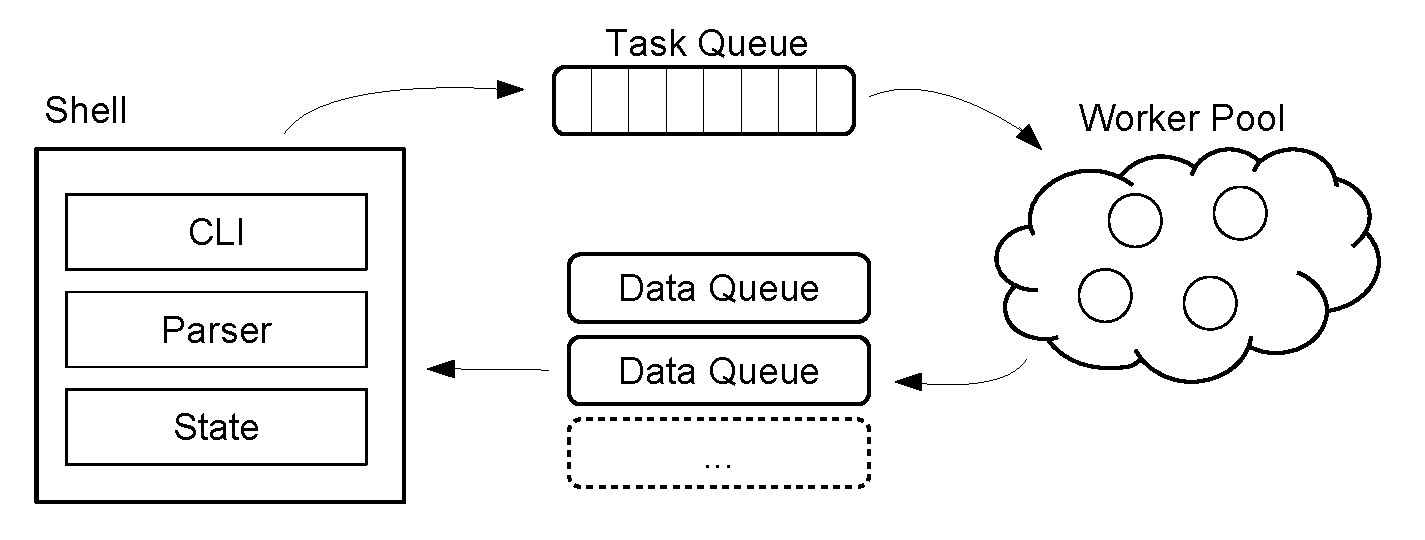
\includegraphics[scale=0.6, keepaspectratio]{system_abstract.pdf}
  \caption{Abstract architecture of the Drift front-end and back-end
           and the interfacing between the two.}
  \label{system-abstract}
\end{figure}

The shell's job is to present the user with a textual interface
and send any valid commands as tasks to the system. Therefor
the shell is \textit{not} part of the system per se. It runs
on the user's machine and connects to the system via network.
This means the user can interface with the system virtually from
anywhere.

Furthermore, as one can see the shell mainly consists of three parts.
All parts and therefor the shell itself are currently implemented
in Java 8 (official version 1.8).
The \textit{command line interface} (CLI) deals with presenting
the shell to the user and handling any input and output from
and to the user. Any input received is passed to the
language parser which was generated using the ANTLR parser
generator (version 4) \cite{antlr}. Additionally in the
parsing layer the shell connects to the service registry which
is not yet shown in the high-level overview of Fig.\ref{system-abstract}.
If any syntactical errors are found or the services do not fit
the specification stored in the service registry, a specific error
message is printed to the screen.

It is important to note however, that in the current implementation
every command entered by the user is fact-checked with the help
of the service registry. This could be optimized by caching any
information retreived about a service in the client shell, therefor
saving round-trips over the network. However, such a caching
infrastructure would, depending on the change rate of the entries
in the service registry, be vulnerable to stale entries. Therefor
some form of cache invalidation or cache coherency protocol would
need to be implemented, updating \textit{all} the client caches
whenever an entry in the service registry changes.
This was considered future work, as will be discussed in the
appropriate chapter, chapter \ref{futurework}.

The third aspect of the shell is the internal state of the session
which consists of two things. A name table that maps the names the
user chose for his session to the names that are used in the system
and the history log for each name.

\subsection{Drift User Interface}
\label{driftui}

To complete the implementation of the \textit{Drift} programming
environment, this section will introduce the system's visualization.
The idea for this visualization is heavily based on the concept
of \textit{immediate feedback} that was introduced in chapter \ref{bretvictor}
as well as on the original idea of a \textit{language of the system}
as introduced in chapter \ref{LanguageOfTheSystem}.

therefore the overall goal of the system's visualization is to
give the user a bird's-eye perspective of the overall system.
This overview should show all the data dependencies that have
been built-up by the user but should also dynamically react
to either new instructions by the user but also new events in
the system itself, e.g. the finishing of a task.

Furthermore this visual representation should not replace the
original shell. It was not supposed to be a visual language
but rather a graphical representation of the data
dependencies created by the user. Using only a textual interface
like the shell, makes it \textit{easy} for the user the built-up
large structures with only a few lines of commands. This can
mislead the user into thinking that the system is still small
and managable when in reality it is a complex dependency graph
containing multiple interconnected data dependencies that
are not easy to grasp. therefore the visual representation
is thought of as a guideline for the user, mirroring her commands
and showing their immediate effects to the overall system.
\newline

Since other workflow systems use a direct acyclic graph (DAG)
to encapsulate and represent the data dependencies as described
by the user, the first idea was to also use a DAG as a dynamic
representation of the system. Whenever the user would enter a new command,
a new vertex would appear in the DAG and whenever a task finished
the system would insert the event into the \texttt{Update} queue
that was introduced in chapter \ref{driftimplementation} and the
DAG would eliminate the corresponding vertex and update its view.

At first this was implemented in exactly that fashion. Unfortunately
this forced the decision whether vertices in the DAG represent
services and were therefore named after the name of the invoked
service, or whether vertices represent the data, being named after
the names given by the user. Although it would've been possible
to allow the user to dynamically switch between both views,
the DAG itself was discarded as a fitting visual representation.
A DAG only describes the dependency aspect of its vertices.
If there is a path from vertex $A$ to vertex $B$ then there is
a dependency between $A$ and $B$. If no such path exists, $A$
are $B$ independent of each other. That is what is captured by
the DAG.

However, the Drift language's core concepts are \textit{data}
and \textit{functionality}. therefore both concepts exist in
the language: \textit{names} (data) and \textit{services}
(functionality). So a visual representation would need to
have two different concepts in order to represent both, names
and services.
Another important aspect of the services orchestrated by the
Drift system is their locality in terms of their inputs, outputs and
state, as was introduced in chapter
\ref{driftimplementation}. This means that no single service
invocation ever has nor needs \textit{any} global information
or global state. Its execution and its outputs only ever depend
on the data contained in its input queues and output is only
ever produced to its own output queue. As was already mentioned
in the last chapter, this is heavily reminiscent of transitions
in a Petri Net because they too only ever consume from their
input places and only ever produce to their output places.

\begin{wrapfigure}{r}{0.3\textwidth}
  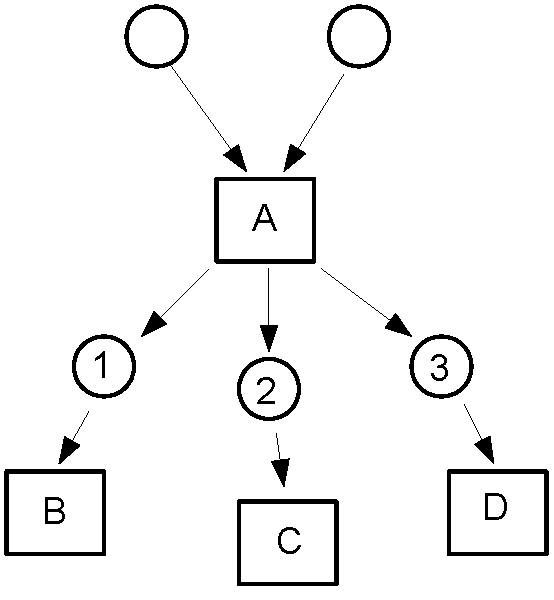
\includegraphics[scale=0.5, keepaspectratio]{pn1.pdf}
  \caption{Rough sketch example of a Petri Net.}
  \label{pn1}
\end{wrapfigure}

Interestingly, since Petri Nets too are based on two core concepts,
namely \textit{places} and \textit{transitions}, they offer different
syntax to talk about both concepts. Figure \ref{pn1} shows a very
rough sketch of the idea of a Petri Net. The Petri Net syntax
uses circles to represent places and squares to represent transitions.
therefore Fig.\ref{pn1} shows a transition $A$ consuming from two
input places and producing to three \textit{different} output places,
$1, 2$ and $3$. These places are then also input places for the
following transitions $B, C$ and $D$ which each only depend
on their single corresponding input place.

This works perfectly fine when the Petri Net is static and modelled
without any dynamically changing parts. However, given the goal
of immediate feedback the Drift shell uses eager-evaluation and
the system is composed \textit{along the way} whenever the user
enters new commands.
therefore it is not possible to infer or predict how many consumers
a given service invocation will have. In the worst-case scenario
all available workers will at some point consume from the
same input data source at the same time. That means that building the
system defensively one would have to add as many output places to any
service invocation as there are workers in the system.

This makes sense in the formalism and realm of Petri Nets because
here, as shown in Fig.\ref{pn1}, transition $B$ could really consume
(meaning eliminate) tokens from place $1$ but not from place $2$.
therefore the \textit{firing} of transition $B$ is completely
independent from the firing of transition $C$ because their inputs
are different. If one would change the given model, having transition
$A$ produce to only a single output place and having transitions
$B, C$ and $D$ all consume from this single place would also
drastically change the semantics of the net. Because in that case
tokens consumed by $B$ would no longer be available to transitions
$C$ and $D$. All three transitions would naturally fight for the
tokens because consuming a token is a destructable action.
\newline

However, given that the output queues in the Drift back end
are implemented using \textit{immutable} Apache Kafka queues, multiple
consumers can consume from the same queue concurrently without
any contention. thereforee, instead of modelling the
producer-consumer relationships between $A$ and $B, C$ and $D$
with different independent output places, a single output
place can be used, as shown by Fig.\ref{pn2}.

\begin{wrapfigure}{l}{0.3\textwidth}
  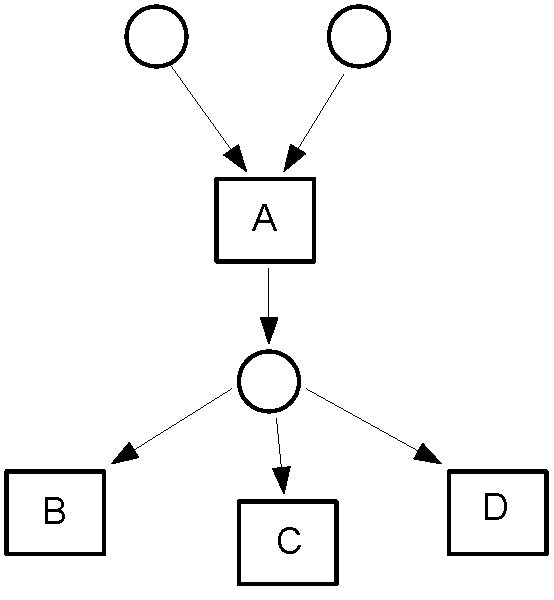
\includegraphics[scale=0.5, keepaspectratio]{pn2.pdf}
  \caption{Minimized net with \textit{different} semantics.}
  \label{pn2}
\end{wrapfigure}

It cannot be highlighted enough that using the original Petri Net
formalism the nets presented in Fig.\ref{pn1} and \ref{pn2} would
have drastically different semantics as explained earlier.
However, the Petri Net \textit{syntax} supports exactly the
same concepts as the Drift language and is therefore a better fit in terms
of visualizing a Drift system than a simple DAG, mapping names
to places and services to transitions. So \textit{only} the
\textit{visual} Petri Net syntax and not the
formalism itself is borrowed in order to visualize a drift system.

So in order implement such a visualization the browser was chosen
as a common platform that allows for ease of use and requires no
installation whatsoever, using HTML, CSS and JavaScript for
implementing the website/web interface.

Figure \ref{gui1} shows the final prototype of that user interface.
As one can see the page is split into three vertical parts. On the left
hand side there is a full Drift shell implementation in the
browser. This embedded shell works exactly like the stand alone
shell that was implemented in Java, as was presented in chapter
\ref{driftshell} and was implemented using the JavaScript
library \textit{jQuery Terminal} \cite{jqueryterminaljs}.

\begin{figure}[h]
  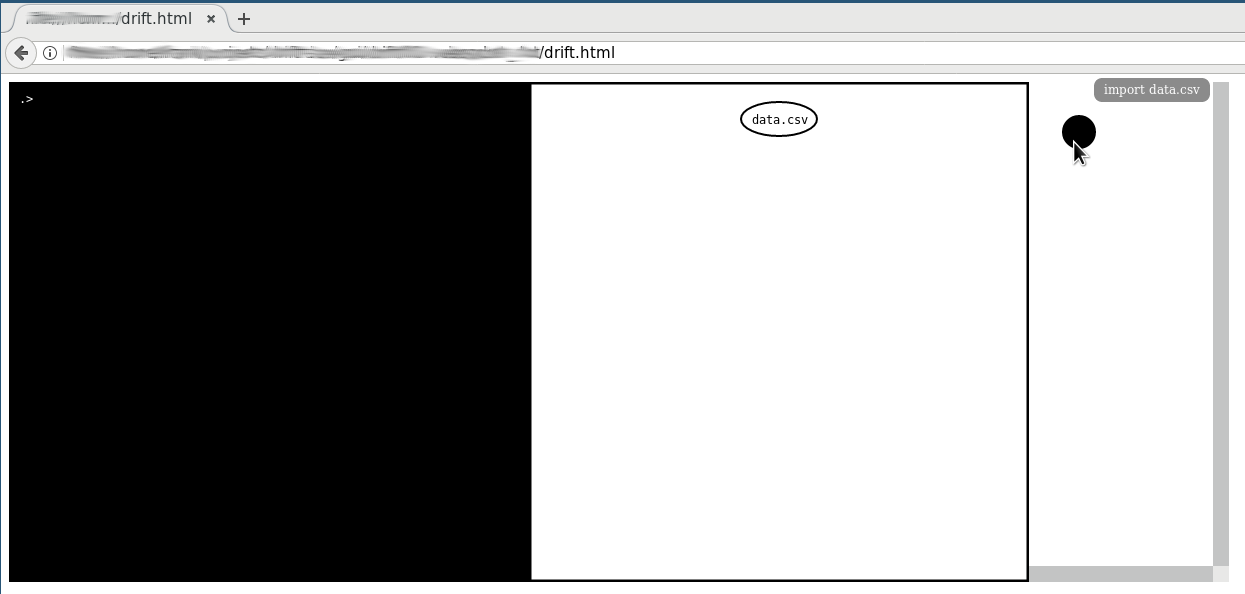
\includegraphics[scale=0.48, keepaspectratio]{gui1.png}
  \caption{Initial state of the system after the import of
           the file \texttt{data.csv}. Imports are also stored
           as events on the the time line.}
  \label{gui1}
\end{figure}

In order for this shell to communicate with the Drift backend
from within the browser a small websocket server was implemented
in Java which only serves as a gateway, forwarding commands from
the shell to the back end and pushing new messages from the
\texttt{Update} queue that was presented in
chapter \ref{errormodel} to the browser using the widely known
\texttt{dot} file format to describe the new graph that should
be printed which resulted from the system update \cite{dotlang},
\cite{dotwiki}.
Since this being a full Drift shell, all the features that were
presented in chapter \ref{driftshell} are present here as well.
Only the \texttt{import} section works differently. Because
one cannot access arbitrary local files from within JavaScript
and the browser, the user needs to select to files which shall
be imported via a GUI wizard, which is the same that is used
for whenever files need to be uploaded on any other website.
User selected files can then be read by the browser and therefore
their content can be uploaded to the Drfit system.

Next to the shell there is an HTML5 canvas containing the graphical
representation of the system using the already introduced Petri Net syntax.
Since most Drift sessions start by importing some local files into the
system, the graph printed on the canvas starts out containing
only unconnected places (circles) with the given name written inside
of them.
The graph is constructed in-memory using a JavaScript library called
\textit{graphlib.js}. The layout of the constructed graph on the
canvas is automatically generated using the \textit{dagre.js}
library and the final printing of the graph onto the canvas is
done using \textit{d3.js} \cite{graphlibjs}, \cite{dagrejs},
\cite{d3js}.

Any new command by the user immediately updates the graph shown
on the canvas. Services used in the command are drawn as transitions
(squares) and connected to their input places accordingly.
If the result of the command is bound to a name, a new place is
drawn and connected to the service as its output place, as
illustrated by Fig.\ref{gui2}. Also a new snapshot of the
current graph is stored and available as an event in the time
line for later review. Furthermore each graph element also
offers a mouse-hover feature, where information about the
service or name is available, e.g. if it was created via an
import.

\begin{figure}[h]
  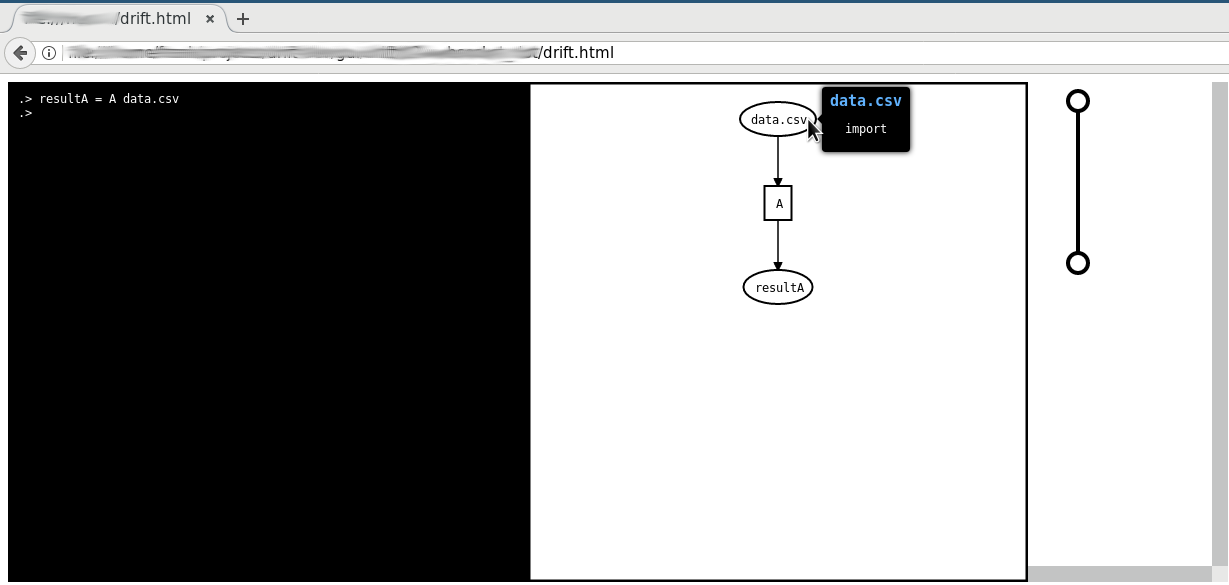
\includegraphics[scale=0.48, keepaspectratio]{gui2.png}
  \caption{A simple service invocation which invokes the
           service in the back and also immediately updates
           the system view.}
  \label{gui2}
\end{figure}

If a service has finished producing its output by sending and
\texttt{EOF} token to its output queue, the update sent to the
\texttt{Update} queue will trigger the removal of the edge
connecting the service to its output place. The same thing
happens when a service consumes an \texttt{EOF} token for one
of its input queues. It sends an event notification to the
\texttt{Update} queue which will send a new graph to the
browser missing the edge between that service and the
corresponding input place.

This means that the user can watch and observe when data has been
finally consume or produced without querying its content. However,
live-querying the streamed data in the shell is still possible.
\newline

But this liveness of the system and its graphical representation
also has its drawbacks. Imagine for example that the user entered
a lot of commands, quickly building up a large graph. Because
of the spacial limitations of the shell, some of the earlier commands
might have already been pushed out of the scope of the shell terminal.
If the user now wants to look up what command created a specific
place, she would have to scroll up, looking for the name and command
that created \textit{that} particular place.

\begin{figure}[h]
  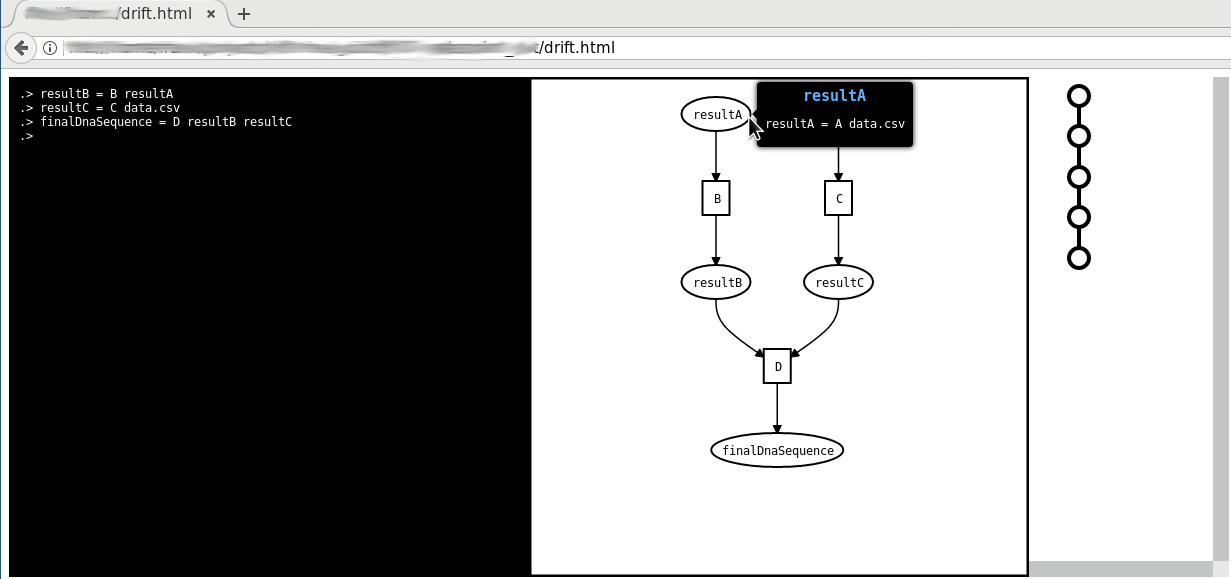
\includegraphics[scale=0.48, keepaspectratio]{gui3.png}
  \caption{Example a more complex dependency graph but because
           service \texttt{A} has already finished, the source
           of \texttt{resultA} is no longer shown in the graph.}
  \label{gui3}
\end{figure}

This is illustrated by Fig.\ref{gui3}. Here the name \texttt{resultA}
does not contain a typical file ending like \texttt{.csv}.
therefore it must have been created by an earlier service invocation
and not an import. But because the service that created this name
has already finished, it was deleted from the system graph and only
its result, \texttt{resultA}, remains. Since then the user has
used the result of her earlier invocation and built-up a
dependency tree in which some parts consume data from that
earlier result.

In order to avoid having to search for the command that created
the name \texttt{resultA}, the graph provides a mouse-hover feature.
If the user hovers over a place, a pop-up will contain the command that
created that place, as is shown in Fig.\ref{gui3}. This is the graphical
equivalent of the history operators \texttt{?} and \texttt{??}
that were introduced in chapter \ref{driftlang}. Of course the
mouse-hover pop-up will contain the original command and input
place names, even when some of the original inputs have now been
overwritten by newer commands.

\begin{figure}[h]
  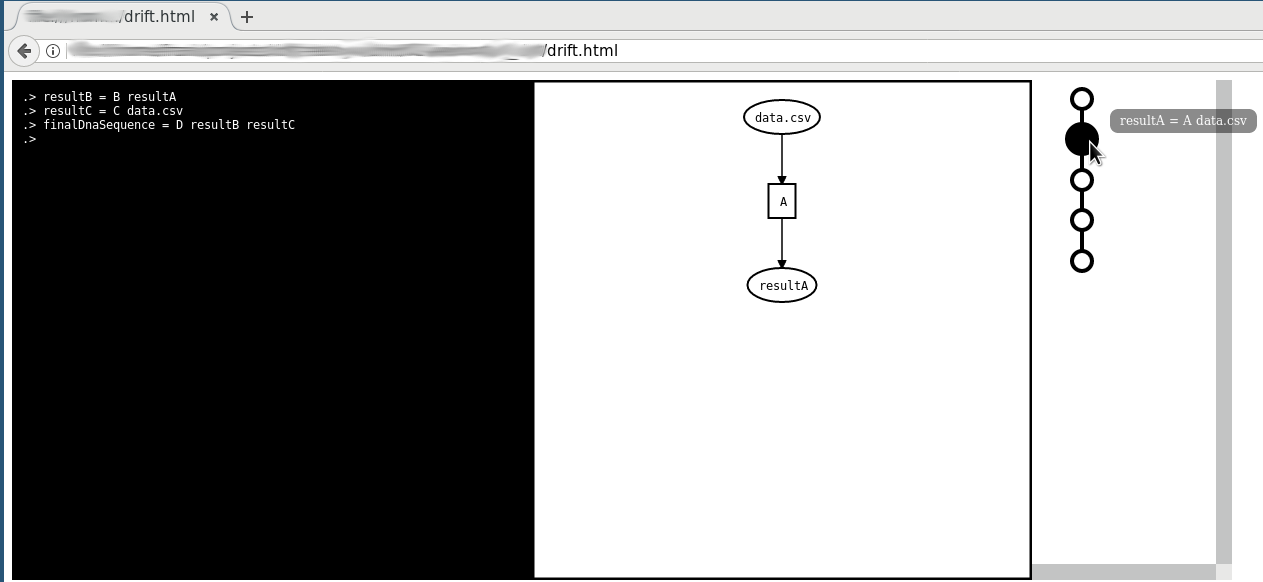
\includegraphics[scale=0.48, keepaspectratio]{gui4.png}
  \caption{Example showing how a mouse-over over the event
           and therefore command that created the resultA name
           shows the snapshot of the system graph at the time
           the command was issued.}
  \label{gui4}
\end{figure}

In order to not only view the command that created a name
but also review the system state at the time the command
that created that name was issued, the user can hover over
the corresponding event in the time line and the canvas
will immediately show the snapshot of the graph that was
stored. therefore old system states are stored and the
user the review the history of the whole system, in the
same way that a user can review old system states in
\textit{Git} as well as \textit{Datomic}, as was introduced
in chapter \ref{git} and \ref{datomic}. The idea of the
event time line is of course heavily inspired by the
time bar presented by Bret Victor, as was introduced in
chapter \ref{bretvictor}.
\newline

So this concludes the Drift user interface, which after
the Drift language and shell and the Drift back end including
the immutable Drift file system, is the last part of the
\textit{Drift Programming Environment}. The Drift UI is
a graphical web interface which offers the same shell that
could also be used as a stand alone shell but additionally
offers a graphical representation of the whole system
using the widely known Petri Net syntax with a slightly
different semantics based on immutable data.

The system graph is updated either by commands of the
user or by updates from the individual and independent
components of the distributed system. thereforee,
although the individual components of the system do
\textit{not} maintain any global state, the UI can still
create the system overview from the individual pieces
of information.



\newpage
\
\newpage


\section{Future Work}
\label{futurework}

\section{Summary}
\label{summary}









\newpage
\ \\
\newpage

\bibliography{0-main}
\bibliographystyle{ieeetr}

% Erzeugen der Selbständigkeitserklärung auf einem neuen Blatt:
\selbstaendigkeitserklaerung{\today}

\end{document}
